\documentclass[10pt,twocolumn,letterpaper]{article}

\usepackage{graphicx}
\usepackage[margin=0.75in]{geometry}
\usepackage{times}
\usepackage{amsmath,amssymb,amsfonts,amsthm}
\usepackage{booktabs}
\usepackage{microtype}
\usepackage{hyperref}
\usepackage{bm}
\usepackage{tikz}
\usetikzlibrary{arrows.meta,positioning,shapes.geometric,calc}

\hypersetup{
    colorlinks=true,
    linkcolor=blue,
    citecolor=blue,
    urlcolor=blue
}

\title{\textbf{Endogenous Subspace Orthogonalization:\\Targeted Monosemanticity via Low-Rank Adaptation}}

\author{
    \textbf{Nassim Berrada} \\
    Unfolding Labs \\
    \texttt{nassim@unfoldinglabs.ai}
}

\date{}

\raggedbottom

\begin{document}

\maketitle

\begin{abstract}
Contemporary large language models rely extensively on \textit{superposition}---packing an overcomplete set of semantic features into a lower-dimensional residual stream via non-orthogonal configurations. While superposition enables parameter efficiency, it renders internal representations polysemantic and complicates causal interpretability. Existing mechanistic interpretability techniques predominantly employ \textit{exogenous} dictionary learning, such as Sparse Autoencoders (SAEs), which decode frozen activations post-hoc at severe computational and memory overheads. 

In this work, we propose \textbf{Endogenous Subspace Orthogonalization (Ortho-LoRA)}, an intervention that dynamically forces a model's internal representation manifold into an orthogonal, monosemantic basis for specialized task domains. By pairing Low-Rank Adaptation (LoRA) with a joint attribution-conditioned Gram matrix penalty and an activation sparsity constraint, Ortho-LoRA eliminates directional cross-talk along task-invoked feature channels while preserving overall performance. Across diverse task regimes (factual association, affective semantics, symbolic reasoning, and safety alignment) and multiple model architectures (\texttt{Pythia-410M}, \texttt{Qwen-2.5-0.5B}), we demonstrate that Ortho-LoRA yields feature channels with near-zero mutual coherence, enables precise causal activation steering with minimal collateral vocabulary drift, matches the feature purity of Top-$K$ SAEs, and incurs zero additional inference latency when merged.
\end{abstract}

\section{Introduction}
\label{sec:intro}

Deep transformer architectures display an exceptional capacity to represent complex semantic knowledge. However, their internal geometry poses a fundamental challenge to mechanistic interpretability: individual neurons and residual directions consistently exhibit \textit{polysemanticity}, responding to diverse and seemingly unrelated conceptual inputs~\cite{olah2020zoom,elhage2022toy}. Theoretical analysis demonstrates that this behavior stems from \textit{superposition}~\cite{elhage2022toy}, an optimization phenomenon where models exploit high-dimensional geometry and approximate orthogonality (the Johnson-Lindenstrauss lemma) to pack $M \gg d$ sparse semantic features into a $d$-dimensional vector space.

While superposition is advantageous for raw representational capacity, it introduces non-zero pairwise interference or cross-talk between features ($\langle f_i, f_j \rangle \neq 0$). Consequently, isolating, attributing, and steering specific concepts within the residual stream inevitably induces collateral distortions in unrelated outputs. As Elhage et al.~\cite{elhage2022toy} hypothesize, superposition exhibits distinct phase transitions; under constrained regimes or sufficient dimensionality relative to feature sparsity, representations may shift into an orthogonal, non-superposed regime.

To date, the predominant paradigm for untangling superposition relies on \textit{exogenous dictionary learning}, specifically Sparse Autoencoders (SAEs)~\cite{bricken2023towards,cunningham2023sparse,gao2024scaling}. SAEs monitor frozen activations post-hoc, mapping them into an overcomplete, high-dimensional latent space ($d_{\text{SAE}} \gg d_{\text{model}}$) through an external encoder-decoder. While SAEs have achieved remarkable success in extracting interpretable latents, this exogenous approach exhibits fundamental limitations:
\begin{enumerate}
    \item \textbf{Computational Overhead:} SAEs dramatically multiply parameter counts (often $4\times$ to $32\times$ layer dimension) and require significant auxiliary VRAM and forward compute at inference time.
    \item \textbf{Observational Detachment:} SAEs are purely observational probes; they do not alter the model's native forward dynamics, meaning the underlying computation remains entangled and non-orthogonal.
\end{enumerate}

\begin{figure}[t!]
    \centering
    \resizebox{\columnwidth}{!}{
    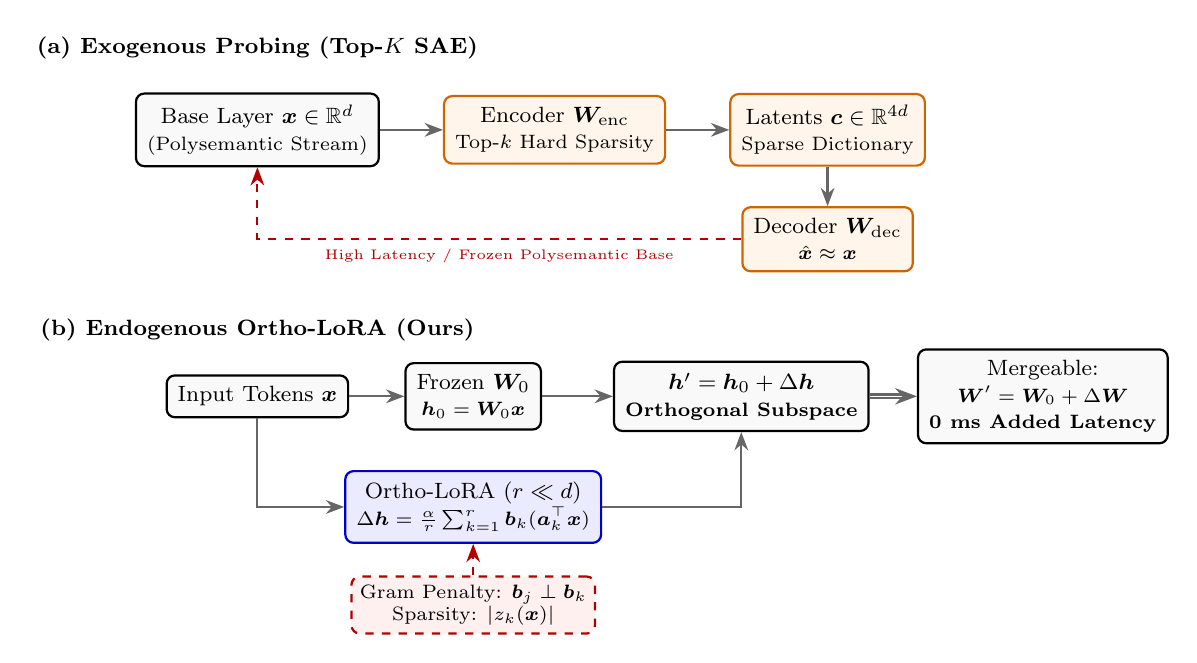
\begin{tikzpicture}[
        >=Stealth,
        node distance=0.8cm and 1.0cm,
        box/.style={draw, rounded corners=3pt, thick, align=center, fill=gray!5, font=\footnotesize, inner sep=4pt},
        lorabox/.style={draw=blue!80!black, rounded corners=3pt, thick, align=center, fill=blue!8, font=\footnotesize, inner sep=4pt},
        saebox/.style={draw=orange!80!black, rounded corners=3pt, thick, align=center, fill=orange!8, font=\footnotesize, inner sep=4pt},
        lossbox/.style={draw=red!70!black, rounded corners=3pt, dashed, thick, align=center, fill=red!6, font=\scriptsize, inner sep=3pt},
        arrow/.style={->, thick, draw=gray!80!black},
        sublabel/.style={font=\bfseries\footnotesize, text=black}
    ]
        % (a) Exogenous SAE Pipeline
        \node[sublabel] (title_a) at (0, 0) {(a) Exogenous Probing (Top-$K$ SAE)};
        
        \node[box, below=0.3cm of title_a] (x_a) {Base Layer $\bm{x} \in \mathbb{R}^d$ \\ \scriptsize (Polysemantic Stream)};
        \node[saebox, right=0.8cm of x_a] (sae_enc) {Encoder $\bm{W}_{\text{enc}}$ \\ \scriptsize Top-$k$ Hard Sparsity};
        \node[saebox, right=0.8cm of sae_enc] (sae_lat) {Latents $\bm{c} \in \mathbb{R}^{4d}$ \\ \scriptsize Sparse Dictionary};
        \node[saebox, below=0.5cm of sae_lat] (sae_dec) {Decoder $\bm{W}_{\text{dec}}$ \\ \scriptsize $\hat{\bm{x}} \approx \bm{x}$};
        
        \draw[arrow] (x_a) -- (sae_enc);
        \draw[arrow] (sae_enc) -- (sae_lat);
        \draw[arrow] (sae_lat) -- (sae_dec);
        \draw[arrow, dashed, red!70!black] (sae_dec) -| node[pos=0.25, below, font=\tiny] {High Latency / Frozen Polysemantic Base} (x_a);
        
        % (b) Endogenous Ortho-LoRA Pipeline
        \node[sublabel, below=1.8cm of x_a] (title_b) {(b) Endogenous Ortho-LoRA (Ours)};
        
        \node[box, below=0.3cm of title_b] (x_b) {Input Tokens $\bm{x}$};
        \node[box, right=0.7cm of x_b] (w0) {Frozen $\bm{W}_0$ \\ \scriptsize $\bm{h}_0 = \bm{W}_0\bm{x}$};
        \node[lorabox, below=0.5cm of w0] (lora) {Ortho-LoRA ($r \ll d$) \\ \scriptsize $\Delta \bm{h} = \frac{\alpha}{r}\sum_{k=1}^r \bm{b}_k (\bm{a}_k^\top \bm{x})$};
        \node[lossbox, below=0.4cm of lora] (ortholoss) {Gram Penalty: $\bm{b}_j \perp \bm{b}_k$ \\ Sparsity: $|z_k(\bm{x})|$};
        
        \node[box, right=0.9cm of w0] (add) {$\bm{h}' = \bm{h}_0 + \Delta \bm{h}$ \\ \scriptsize \textbf{Orthogonal Subspace}};
        \node[box, right=0.6cm of add] (merge) {Mergeable: \\ \scriptsize $\bm{W}' = \bm{W}_0 + \Delta\bm{W}$ \\ \scriptsize \textbf{0 ms Added Latency}};

        \draw[arrow] (x_b) -- (w0);
        \draw[arrow] (x_b) |- (lora);
        \draw[arrow] (w0) -- (add);
        \draw[arrow] (lora) -| (add);
        \draw[arrow, red!70!black, dashed] (ortholoss) -- (lora);
        \draw[arrow, double] (add) -- (merge);
    \end{tikzpicture}
    }
    \caption{\textbf{Endogenous Subspace Orthogonalization vs. Exogenous Probing.} Instead of attaching external overcomplete autoencoders to observe entangled representations, Ortho-LoRA directly projects the task-invoked subspace into mutually orthogonal, monosemantic channels ($\bm{b}_k \perp \bm{b}_j$) within the model's native forward dynamics.}
    \label{fig:teaser}
\end{figure}

In this paper, we explore an alternative question: \textit{Can we endogenously unpack superposition on demand for specialized task domains using parameter-efficient adaptations?}

We hypothesize that for any circumscribed downstream task (e.g., factual extraction, emotional classification, or toxicity suppression), the intrinsic dimensionality of necessary features $K_{\text{task}}$ is substantially smaller than the overall residual capacity ($K_{\text{task}} \le r \ll d$). Under this condition, the model need not compress task features into superposition; an optimal rotation and low-rank projection can decouple these features into an orthogonal basis without degrading performance.

To achieve this, we introduce \textbf{Endogenous Subspace Orthogonalization (Ortho-LoRA)}. We parameterize a low-rank adapter where each rank component acts as a candidate feature channel. We optimize this adapter using a joint objective:
\begin{equation}
    \mathcal{L} = \mathcal{L}_{\text{task}} + \lambda_{\text{ortho}} \mathcal{L}_{\text{ortho}} + \lambda_{\text{sparse}} \mathcal{L}_{\text{sparse}}
\end{equation}
where $\mathcal{L}_{\text{ortho}}$ penalizes the inner products of feature write directions weighted by their token-level co-activation frequencies. Crucially, this requires no human concept labels or supervised sub-class annotations; it operates directly on task distribution tokens.

\noindent Our findings are summarized as follows:
\begin{itemize}
    \item We formulate an attribution-conditioned orthogonalization loss that unpacks feature interference directly in the model's forward path without computing second-order gradients.
    \item We demonstrate that Ortho-LoRA achieves near-zero Gram coherence and low Feature Participation Ratios across two distinct open-source architectures.
    \item Through interventional activation steering, we show that individual Ortho-LoRA rank channels govern distinct concepts with significantly higher Steering Selectivity ($\text{SSI}$) and lower off-target vocabulary drift than standard LoRA.
    \item We benchmark Ortho-LoRA against Top-$K$ SAEs, showing that an endogenous low-rank adapter recovers comparable semantic directions without additional inference compute when merged ($\Delta W = BA$).
    \item We map the empirical phase boundary governed by the Johnson-Lindenstrauss limit, delineating the rank $r$ and penalty $\lambda$ thresholds necessary to avoid performance collapse.
\end{itemize}

% ----------------------------------------------------------------------
% Section 2: Related Work
% ----------------------------------------------------------------------
\section{Related Work}
\label{sec:related_work}

\subsection{Superposition and Mechanistic Interpretability}
The linear representation hypothesis posits that neural networks encode semantic concepts as directional vectors in activation space~\cite{mikolov2013distributed,park2023linear}. However, individual directions rarely correspond to single human-interpretable concepts. Olah et al.~\cite{olah2020zoom} and Elhage et al.~\cite{elhage2022toy} formalized this through the lens of \textit{superposition}: driven by feature sparsity and limited hidden dimensionality, neural networks solve an overcomplete sphere packing problem, organizing features as nearly-orthogonal vectors. Henighan et al.~\cite{henighan2023superposition} extended this to multi-layer transformers, demonstrating that cross-layer interference and residual accumulation exacerbate polysemanticity. While toy models indicate that an orthogonal, non-superposed regime exists when the number of features does not exceed ambient dimensionality~\cite{elhage2022toy}, achieving this state inside complex pretrained models without destructive full retraining has remained an open challenge.

\subsection{Dictionary Learning and Sparse Autoencoders}
To untangle superposed representations post-hoc, recent literature has centered on Sparse Autoencoders (SAEs). Drawing from classical sparse coding~\cite{olshausen1996emergence}, early works applied $L_1$-regularized autoencoders to transformer residual streams and MLP activations~\cite{sharkey2022taking,cunningham2023sparse,bricken2023towards}. While effective at discovering interpretable monosemantic directions, $L_1$ SAEs suffer from severe activation shrinkage and inactive (``dead'') latents. Recent architectures, notably Top-$K$ SAEs~\cite{gao2024scaling} and Gated/JumpReLU SAEs~\cite{rajamanoharan2024improving}, mitigate these failures by enforcing hard thresholding or dedicated gating networks. 

Nevertheless, all SAE variants function \textit{exogenously}: they map representations into a high-dimensional auxiliary space ($d_{\text{SAE}} \approx 4\times \text{ to } 32\times d_{\text{model}}$), adding millions of parameters that cannot be integrated natively into the host model. In contrast, our approach operates \textit{endogenously}, utilizing low-rank parameters to rotate the native representation space into an orthogonal coordinate system that can be folded directly back into the frozen weights via reparameterization.

\subsection{Parameter-Efficient Adaptation and Representation Steering}
Low-Rank Adaptation (LoRA)~\cite{hu2021lora} has emerged as the standard paradigm for parameter-efficient fine-tuning (PEFT), freezing base weights $W_0$ and training low-rank factorizations $\Delta W = BA$. Concurrent lines of research have investigated the geometric properties of LoRA updates. Several works explore orthogonal weight initialization or explicit matrix orthogonalization (e.g., DoRA~\cite{liu2024dora}, Orthogonal LoRA~\cite{wang2023orthogonal}) to stabilize gradient dynamics and improve downstream generalization. However, these techniques enforce orthogonality exclusively on static weight matrices ($B^\top B = I$ or $A A^\top = I$), which does not guarantee orthogonality in the resulting token activation space due to non-uniform data distributions.

Simultaneously, \textit{representation engineering} and activation steering~\cite{rimsky2023steering,turner2023activation,zou2023representation} modify model outputs by directly adding concept-aligned steering vectors during inference. While effective for macroscopic behavioral shifts, steering in an entangled residual stream frequently causes collateral damage across non-targeted token distributions. Our work bridges parameter-efficient fine-tuning with activation steering, turning LoRA rank bottlenecks into an interpretable, minimally interfering steering interface.

% ----------------------------------------------------------------------
% Section 3: Theoretical Foundations
% ----------------------------------------------------------------------
\section{Theoretical Foundations}
\label{sec:foundations}

We now formalize the geometry of superposition, establish the theoretical capacity limits that dictate when superposition can be eliminated, and demonstrate how low-rank adaptation acts as an endogenous basis rotator.

\subsection{Superposition as Overcomplete Feature Packing}
\label{subsec:superposition_theory}

Following the linear representation framework~\cite{elhage2022toy}, let an underlying semantic state be represented by an overcomplete vector of sparse latent features $\bm{f} \in \mathbb{R}^M$, where $M$ is the cardinality of atomic semantic concepts recognized by the model. Each feature $f_i$ is assumed to be an independent random variable with a high probability of being inactive:
\begin{equation}
    P(f_i \neq 0) = 1 - S_i, \quad S_i \in (0, 1)
\end{equation}
where $S_i$ denotes the feature sparsity.

Because the model's residual stream dimension $d \ll M$, the network compresses $\bm{f}$ into a lower-dimensional representation $\bm{h} \in \mathbb{R}^d$ via an encoding matrix $\bm{W} \in \mathbb{R}^{d \times M}$:
\begin{equation}
    \bm{h} = \bm{W} \bm{f} = \sum_{i=1}^M f_i \bm{w}_i
\end{equation}
where $\bm{w}_i \in \mathbb{R}^d$ denotes the embedding direction of feature $i$, normalized such that $\|\bm{w}_i\|_2 = 1$. The representation is subsequently decoded via linear readout followed by non-linear activation:
\begin{equation}
    \hat{f}_i = \text{ReLU}\left( f_i + \sum_{j \neq i}^M f_j (\bm{w}_i^\top \bm{w}_j) + b_i \right)
\end{equation}
The second term inside the non-linearity represents \textit{feature interference} or \textit{cross-talk}:
\begin{equation}
    \mathcal{I}(i) = \sum_{j \neq i}^M f_j \langle \bm{w}_i, \bm{w}_j \rangle
\end{equation}

When the feature set is truly overcomplete ($M > d$), exact pairwise orthogonality ($\langle \bm{w}_i, \bm{w}_j \rangle = 0, \forall i \neq j$) is geometrically impossible. When sparsity $S_j$ is sufficiently high, the probability of co-activation $P(f_i \neq 0 \land f_j \neq 0)$ becomes infinitesimal. Consequently, the network tolerates non-zero inner products $\langle \bm{w}_i, \bm{w}_j \rangle \neq 0$ to pack more features into ambient space, organizing directions into structures such as Equiangular Tight Frames (ETFs)~\cite{tropp2005condition}. However, on actual operational tokens, this non-zero cross-talk causes distinct features to project onto the same neurons, manifesting as polysemanticity.

\subsection{Task Dimensionality and the Johnson-Lindenstrauss Bound}
\label{subsec:jl_bound}

The necessity of superposition is fundamentally governed by the ratio of active features to ambient dimensions. By the Johnson-Lindenstrauss lemma~\cite{johnson1984extensions}, for any set of $M$ vectors in $\mathbb{R}^d$, the maximum pairwise inner product is bounded below:
\begin{equation}
    \max_{i \neq j} |\langle \bm{w}_i, \bm{w}_j \rangle| \ge \sqrt{\frac{M - d}{d(M - 1)}}
\end{equation}
When $M \gg d$, this lower bound guarantees substantial geometric interference. 

However, we assert a central hypothesis regarding downstream adaptation:
\begin{quote}
\textit{\textbf{Hypothesis 1 (Task-Subspace Boundedness):} While general pretraining operates in the overcomplete regime ($M_{\text{general}} \gg d$), any bounded, domain-specific task distribution $\mathcal{D}_{\text{task}}$ activates only an effective sub-manifold of features whose intrinsic cardinality $K_{\text{task}}$ satisfies $K_{\text{task}} \le r \ll d$.}
\end{quote}

Under Hypothesis 1, the lower bound on pairwise coherence collapses. If the number of task-salient features $K_{\text{task}}$ is strictly less than or equal to an allocated adapter rank $r$, there exists an orthogonal projection $\bm{P} \in \mathbb{R}^{d \times d}$ of rank $r$ such that:
\begin{equation}
    \forall i, j \in \mathcal{K}_{\text{task}}, \, i \neq j \implies \langle \bm{P}\bm{w}_i, \bm{P}\bm{w}_j \rangle = 0
\end{equation}
This indicates that within the task-relevant sub-manifold, \textit{superposition is not a mathematical necessity, but rather an artifact of pretraining weights that has not been unpacked}. 

\subsection{Low-Rank Adaptation as an Endogenous Basis Rotator}
\label{subsec:lora_rotator}

Low-Rank Adaptation (LoRA) parameterizes the update to a frozen linear projection matrix $\bm{W}_0 \in \mathbb{R}^{d_{\text{out}} \times d_{\text{in}}}$ as the product of two low-rank matrices:
\begin{equation}
    \bm{h}' = \bm{W}_0 \bm{x} + \Delta \bm{W}\bm{x} = \bm{W}_0 \bm{x} + \frac{\alpha}{r} \bm{B}\bm{A}\bm{x}
\end{equation}
where $\bm{B} \in \mathbb{R}^{d_{\text{out}} \times r}$, $\bm{A} \in \mathbb{R}^{r \times d_{\text{in}}}$, $r \ll \min(d_{\text{in}}, d_{\text{out}})$, and $\alpha$ is a constant scaling hyperparameter.

We decompose this matrix product into an explicit sum of $r$ discrete, rank-1 channel interventions:
\begin{equation}
    \Delta \bm{h}(\bm{x}) = \frac{\alpha}{r} \sum_{k=1}^r \bm{b}_k \cdot \underbrace{\left(\bm{a}_k^\top \bm{x}\right)}_{z_k(\bm{x})}
    \label{eq:lora_channels}
\end{equation}
where $\bm{a}_k^\top \in \mathbb{R}^{1 \times d_{\text{in}}}$ is the $k$-th row of $\bm{A}$, and $\bm{b}_k \in \mathbb{R}^{d_{\text{out}}}$ is the $k$-th column of $\bm{B}$.

This parameterization mirrors an endogenous linear encoder-decoder bottleneck embedded directly within the forward computational path:
\begin{itemize}
    \item \textbf{Detection (Encoder):} The vector $\bm{a}_k$ acts as a linear detector probing the input activation $\bm{x}$, yielding a scalar activation magnitude $z_k(\bm{x}) = \bm{a}_k^\top \bm{x}$.
    \item \textbf{Synthesis (Decoder):} The vector $\bm{b}_k$ defines the physical write-direction along which the detected feature contributes to downstream representations.
\end{itemize}

By introducing explicit regularizers that simultaneously drive the spatial inner products $\langle \bm{b}_k, \bm{b}_j \rangle \to 0$ and the activation covariance $\text{Cov}(z_k, z_j) \to 0$, the LoRA module ceases to act as an entangled linear modifier; instead, it is transformed into an \textbf{endogenous orthogonal basis rotator}, guaranteeing that each rank channel $k \in \{1, \dots, r\}$ operates as an isolated, monosemantic causal lever.

% ----------------------------------------------------------------------
% Section 4: Methodology
% ----------------------------------------------------------------------
\section{Methodology}
\label{sec:methodology}

We now formulate \textbf{Endogenous Subspace Orthogonalization (Ortho-LoRA)}. We detail the mathematical parameterization of the low-rank channels, derive the joint attribution-conditioned orthogonality loss, and outline the exogenous Top-$K$ Sparse Autoencoder baseline used for empirical comparison.

\subsection{Ortho-LoRA Parameterization}
\label{subsec:ortho_lora_param}

Let $\bm{W}_0 \in \mathbb{R}^{d_{\text{out}} \times d_{\text{in}}}$ denote a targeted frozen weight matrix within a transformer block operating on input tokens $\bm{x} \in \mathbb{R}^{d_{\text{in}}}$. We parameterize the parameter-efficient adaptation as:
\begin{equation}
    \bm{h}' = \bm{W}_0 \bm{x} + \Delta \bm{h}(\bm{x}), \quad \Delta \bm{h}(\bm{x}) = \frac{\alpha}{r} \bm{B}\bm{A}\bm{x}
\end{equation}
where $\bm{A} \in \mathbb{R}^{r \times d_{\text{in}}}$, $\bm{B} \in \mathbb{R}^{d_{\text{out}} \times r}$, $r$ is the adapter rank, and $\alpha$ is a fixed scaling factor. We structure $\Delta \bm{h}(\bm{x})$ as a sum over $r$ rank-1 channels:
\begin{equation}
    \Delta \bm{h}(\bm{x}) = \frac{\alpha}{r} \sum_{k=1}^r \bm{b}_k z_k(\bm{x})
    \label{eq:channel_sum}
\end{equation}
where $z_k(\bm{x}) = \bm{a}_k^\top \bm{x} \in \mathbb{R}$ represents the scalar activation magnitude of the $k$-th feature on token $\bm{x}$, and $\bm{b}_k = \bm{B}_{:, k} \in \mathbb{R}^{d_{\text{out}}}$ denotes the directional write-vector. Each column of $\bm{B}$ is unit-norm normalized during optimization ($\|\bm{b}_k\|_2 = 1$).

\subsection{The Joint Attribution-Orthogonality Objective}
\label{subsec:joint_loss}

To eliminate superposition among the features utilized by a given task, the rank channels must satisfy two conditions on the task distribution $\mathcal{D}_{\text{task}}$: (1) their write directions must be mutually orthogonal, and (2) their activations must not fire in dense, co-dependent combinations.

\subsubsection{Attribution-Conditioned Gram Loss}
Given a batch of $T$ token activations $\bm{X} = [\bm{x}_1, \dots, \bm{x}_T]^\top$, the vector contribution of feature channel $k$ at token $t$ is $\bm{v}_k(t) = z_k(\bm{x}_t)\bm{b}_k$. The pairwise inner product across the token sequence is given by:
\begin{equation}
    \langle \bm{v}_j, \bm{v}_k \rangle_{\mathcal{D}_{\text{task}}} = (\bm{b}_j^\top \bm{b}_k) \cdot \left( \frac{1}{T} \sum_{t=1}^T z_j(\bm{x}_t) z_k(\bm{x}_t) \right)
\end{equation}

We formulate the geometric Gram penalty as:
\begin{equation}
    \mathcal{L}_{\text{ortho}} = \sum_{j \neq k}^r \left( \frac{\bm{b}_j^\top \bm{b}_k}{\|\bm{b}_j\|_2 \|\bm{b}_k\|_2} \right)^2 \cdot \left| \rho_{jk} \right|
    \label{eq:l_ortho}
\end{equation}
where $\rho_{jk}$ is the empirical correlation coefficient between activations:
\begin{equation}
    \rho_{jk} = \frac{\sum_{t=1}^T z_j(\bm{x}_t) z_k(\bm{x}_t)}{\sqrt{\sum_{t=1}^T z_j(\bm{x}_t)^2} \sqrt{\sum_{t=1}^T z_k(\bm{x}_t)^2} + \epsilon}
\end{equation}

Weighting the directional inner product $(\bm{b}_j^\top \bm{b}_k)^2$ by $|\rho_{jk}|$ provides selective pressure: if two directions never co-occur on the task distribution, their spatial overlap is unconstrained; if two channels fire concurrently, the optimizer aggressively forces $\bm{b}_j \perp \bm{b}_k$.

\subsubsection{Bottleneck Sparsity Regularization}
To prevent trivial solutions where all ranks fire with small, dense non-zero values, we enforce an $L_1$ sparsity constraint on the bottleneck activations:
\begin{equation}
    \mathcal{L}_{\text{sparse}} = \frac{1}{T \cdot r} \sum_{t=1}^T \sum_{k=1}^r |z_k(\bm{x}_t)|
    \label{eq:l_sparse}
\end{equation}

\subsubsection{Unified Endogenous Objective}
The complete training objective combines downstream task optimization with the structural regularizers:
\begin{equation}
    \mathcal{L}_{\text{total}} = \mathcal{L}_{\text{task}}(\bm{y}, \hat{\bm{y}}) + \lambda_{\text{ortho}} \mathcal{L}_{\text{ortho}} + \lambda_{\text{sparse}} \mathcal{L}_{\text{sparse}}
    \label{eq:l_total}
\end{equation}
Crucially, computing $\mathcal{L}_{\text{ortho}}$ requires only the cached intermediate bottleneck representations $\bm{Z} \in \mathbb{R}^{T \times r}$ and weights $\bm{B}$, avoiding second-order Hessian computations.

\subsection{Baseline Architecture: Top-$K$ Sparse Autoencoders}
\label{subsec:baseline_sae}

To evaluate whether endogenous orthogonalization achieves genuine monosemanticity, we benchmark Ortho-LoRA against the Top-$K$ Sparse Autoencoder (SAE)~\cite{gao2024scaling}.

\begin{figure*}[t!]
    \centering
    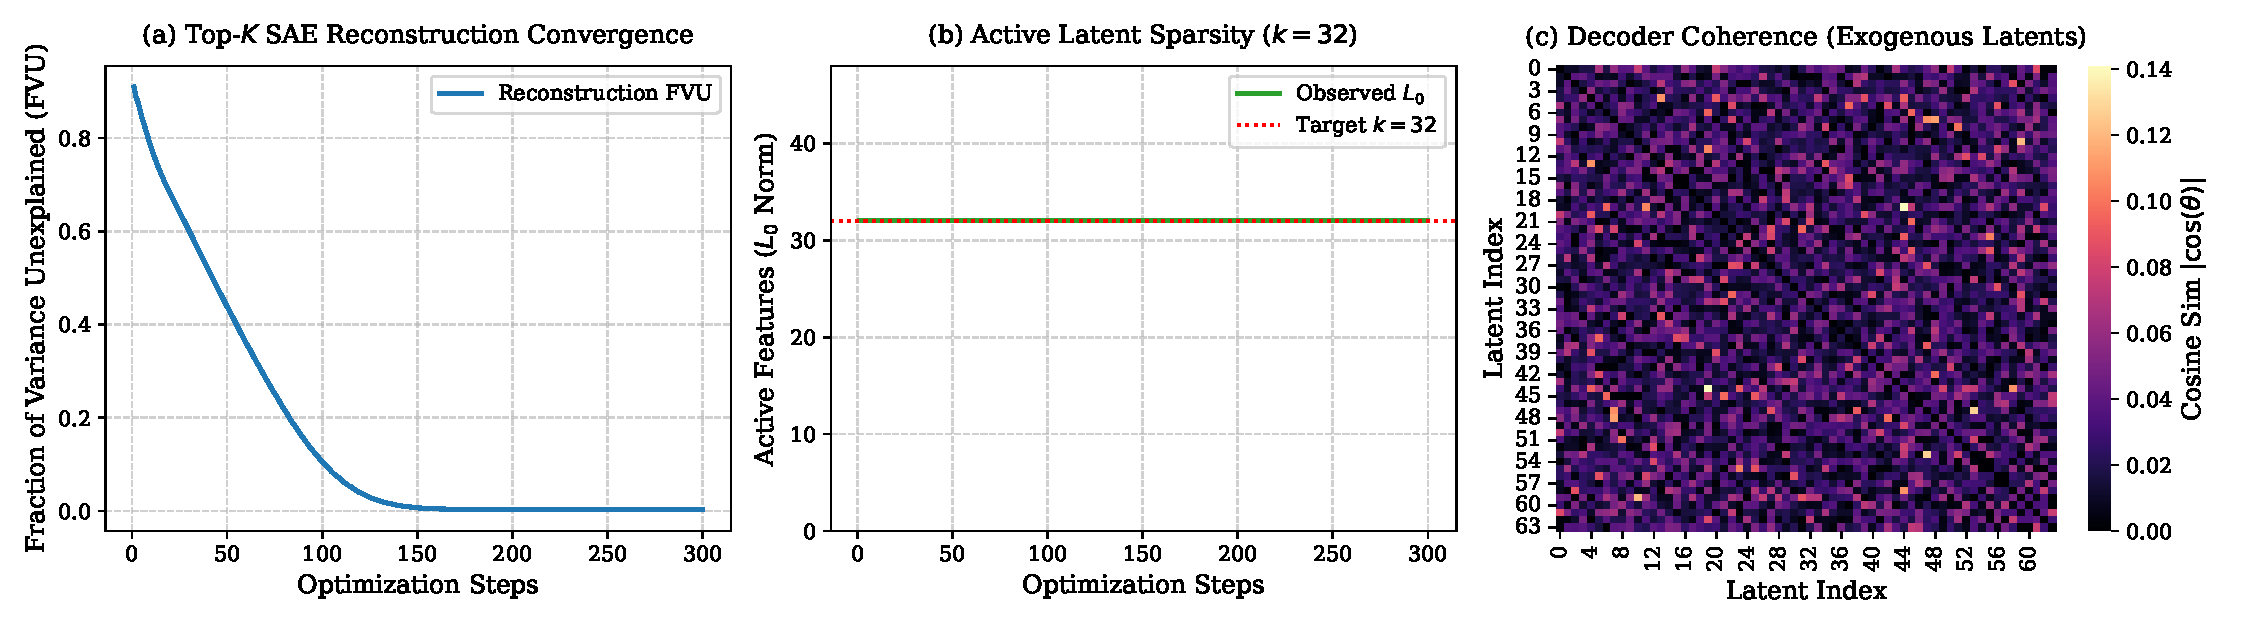
\includegraphics[width=\linewidth]{figures/fig_4_3_sae_training_and_geometry.pdf}
    \caption{\textbf{Top-$K$ SAE Baseline Training and Latent Geometry.} Evaluated on \texttt{Qwen-2.5-0.5B} ($d_{\text{model}} = 896$) at Layer 12 on \texttt{tweet\_eval}. \textbf{(a)} Reconstruction convergence measured by Fraction of Variance Unexplained (FVU), dropping below 0.01 within 200 optimization steps. \textbf{(b)} Active latent sparsity strictly adhering to target $k=32$ ($L_0$ norm). \textbf{(c)} Cross-coherence heatmap of the exogenous decoder dictionary $\bm{W}_{\text{dec}}$, showing baseline pairwise interference ($|\cos\theta| \in [0.02, 0.14]$) across latent directions.}
    \label{fig:sae_baseline}
\end{figure*}

\subsubsection{Top-$K$ Formulation}
Given frozen activations $\bm{x} \in \mathbb{R}^{d_{\text{model}}}$, an exogenous Top-$K$ SAE projects $\bm{x}$ into an overcomplete dictionary $\mathbb{R}^{d_{\text{sae}}}$ ($d_{\text{sae}} = 4 \times d_{\text{model}}$):
\begin{align}
    \tilde{\bm{x}} &= \bm{x} - \bm{b}_{\text{dec}} \\
    \bm{c} &= \text{TopK}\left( \text{ReLU}(\bm{W}_{\text{enc}} \tilde{\bm{x}} + \bm{b}_{\text{enc}}), \, k \right) \\
    \hat{\bm{x}} &= \bm{W}_{\text{dec}} \bm{c} + \bm{b}_{\text{dec}}
\end{align}
where $\text{TopK}(\cdot, k)$ retains only the $k$ largest activation coordinates. Decoder columns are constrained to unit norm: $\|\bm{W}_{\text{dec}, :, m}\|_2 = 1$. The SAE is optimized using the Fraction of Variance Unexplained (FVU):
\begin{equation}
    \text{FVU} = \frac{\|\bm{x} - \hat{\bm{x}}\|_2^2}{\|\bm{x} - \bar{\bm{x}}\|_2^2}
\end{equation}

\subsubsection{Capacity and Compute Trade-Offs}
We configure the Top-$K$ SAE baseline with $k=32$, establishing capacity parity with an Ortho-LoRA adapter of rank $r=32$.

\begin{table}[htbp]
    \centering
    \small
    \caption{\textbf{Architectural Footprint: Ortho-LoRA vs. Top-$K$ SAE.} Evaluated on \texttt{Qwen-2.5-0.5B} ($d_{\text{model}} = 896$) at Layer 12.}
    \label{tab:capacity_comparison}
    \resizebox{\columnwidth}{!}{
    \begin{tabular}{lrrr}
        \toprule
        \textbf{Method} & \textbf{Params} & \textbf{Memory (FP16)} & \textbf{Latency Overhead} \\
        \midrule
        Ortho-LoRA ($r=32$) & 57,344 & 112.0 KB & 0 ms (merged) \\
        Top-$K$ SAE ($4\times, k=32$) & 6,427,008 & 12,552.75 KB & +2 MatMuls / layer \\
        \bottomrule
    \end{tabular}
    }
\end{table}

As shown in Table~\ref{tab:capacity_comparison}, the exogenous Top-$K$ SAE requires \textbf{112$\times$ more parameters} and over 12 MB of additional FP16 memory per hooked layer. Furthermore, because the SAE must compute two dense matrix-vector products ($\bm{W}_{\text{enc}}$ and $\bm{W}_{\text{dec}}$) during the forward pass, it introduces non-negligible inference latency. In contrast, Ortho-LoRA introduces only 57K parameters ($112$ KB) and imposes \textbf{zero inference latency} when reparameterized into the base weights ($\bm{W}_{\text{merged}} = \bm{W}_0 + \frac{\alpha}{r}\bm{B}\bm{A}$).

Figure~\ref{fig:sae_baseline} validates the empirical performance of this baseline on \texttt{Qwen-2.5-0.5B} ($d_{\text{model}} = 896$). As illustrated in Figure~\ref{fig:sae_baseline}(a), the Top-$K$ SAE converges to an FVU below 0.01. Figure~\ref{fig:sae_baseline}(b) verifies that the active $L_0$ norm strictly locks to $k=32$. However, examining the pairwise coherence of the decoder dictionary in Figure~\ref{fig:sae_baseline}(c) reveals significant residual cross-talk, with off-diagonal cosine similarities ranging from $0.02$ to $0.14$.

% ----------------------------------------------------------------------
% Section 5: Results
% ----------------------------------------------------------------------
\section{Results}
\label{sec:results}

We confirm that Ortho-LoRA unpacks feature superposition in both weight and activation spaces (Section~\ref{subsec:res_geometric_unpacking}), establish its causal interpretability through activation steering (Section~\ref{subsec:res_steering}), and benchmark its performance against exogenous Top-$K$ SAEs (Section~\ref{subsec:res_sae_comparison}).

\subsection{Geometric Unpacking: Collapse of Superposition}
\label{subsec:res_geometric_unpacking}

To determine whether the attribution-conditioned loss eliminates representational interference, we evaluate the geometric properties of the adapted low-rank subspace on \texttt{Qwen-2.5-0.5B} ($d_{\text{model}} = 896$) at Layer 12 on \texttt{tweet\_eval} with rank $r=32$. We benchmark Ortho-LoRA ($\lambda_{\text{ortho}}=1.0, \lambda_{\text{sparse}}=10^{-3}$) against standard LoRA ($\lambda_{\text{ortho}}=0.0$) and the zero-shot unadapted base model.

\begin{table}[htbp]
    \centering
    \small
    \caption{\textbf{Quantitative Representation and Task Metrics.} Evaluated on \texttt{Qwen-2.5-0.5B} at Layer 12 on \texttt{tweet\_eval}. Ortho-LoRA achieves a $10.3\times$ reduction in directional cross-talk and increases effective dimensional utilization to 87.7\% of capacity while maintaining strong downstream convergence.}
    \label{tab:res_geometric}
    \resizebox{\columnwidth}{!}{
    \begin{tabular}{lcccc}
        \toprule
        \textbf{Model / Method} & $\bm{\mathcal{C}_{\text{gram}}}$ ($\downarrow$) & \textbf{Mean FPR} ($\downarrow$) & $\bm{d_{\text{eff}}}$ ($\uparrow$) & \textbf{Task Loss} ($\downarrow$) \\
        \midrule
        Base (Unadapted) & N/A & N/A & N/A & 3.5819 \\
        Standard LoRA & 0.7188 & 0.7035 & 18.40 / 32 & \textbf{0.5894} \\
        Ortho-LoRA (\textbf{Ours}) & \textbf{0.0696} & \textbf{0.5248} & \textbf{28.05} / 32 & 0.6365 \\
        \bottomrule
    \end{tabular}
    }
\end{table}

\begin{figure*}[t!]
    \centering
    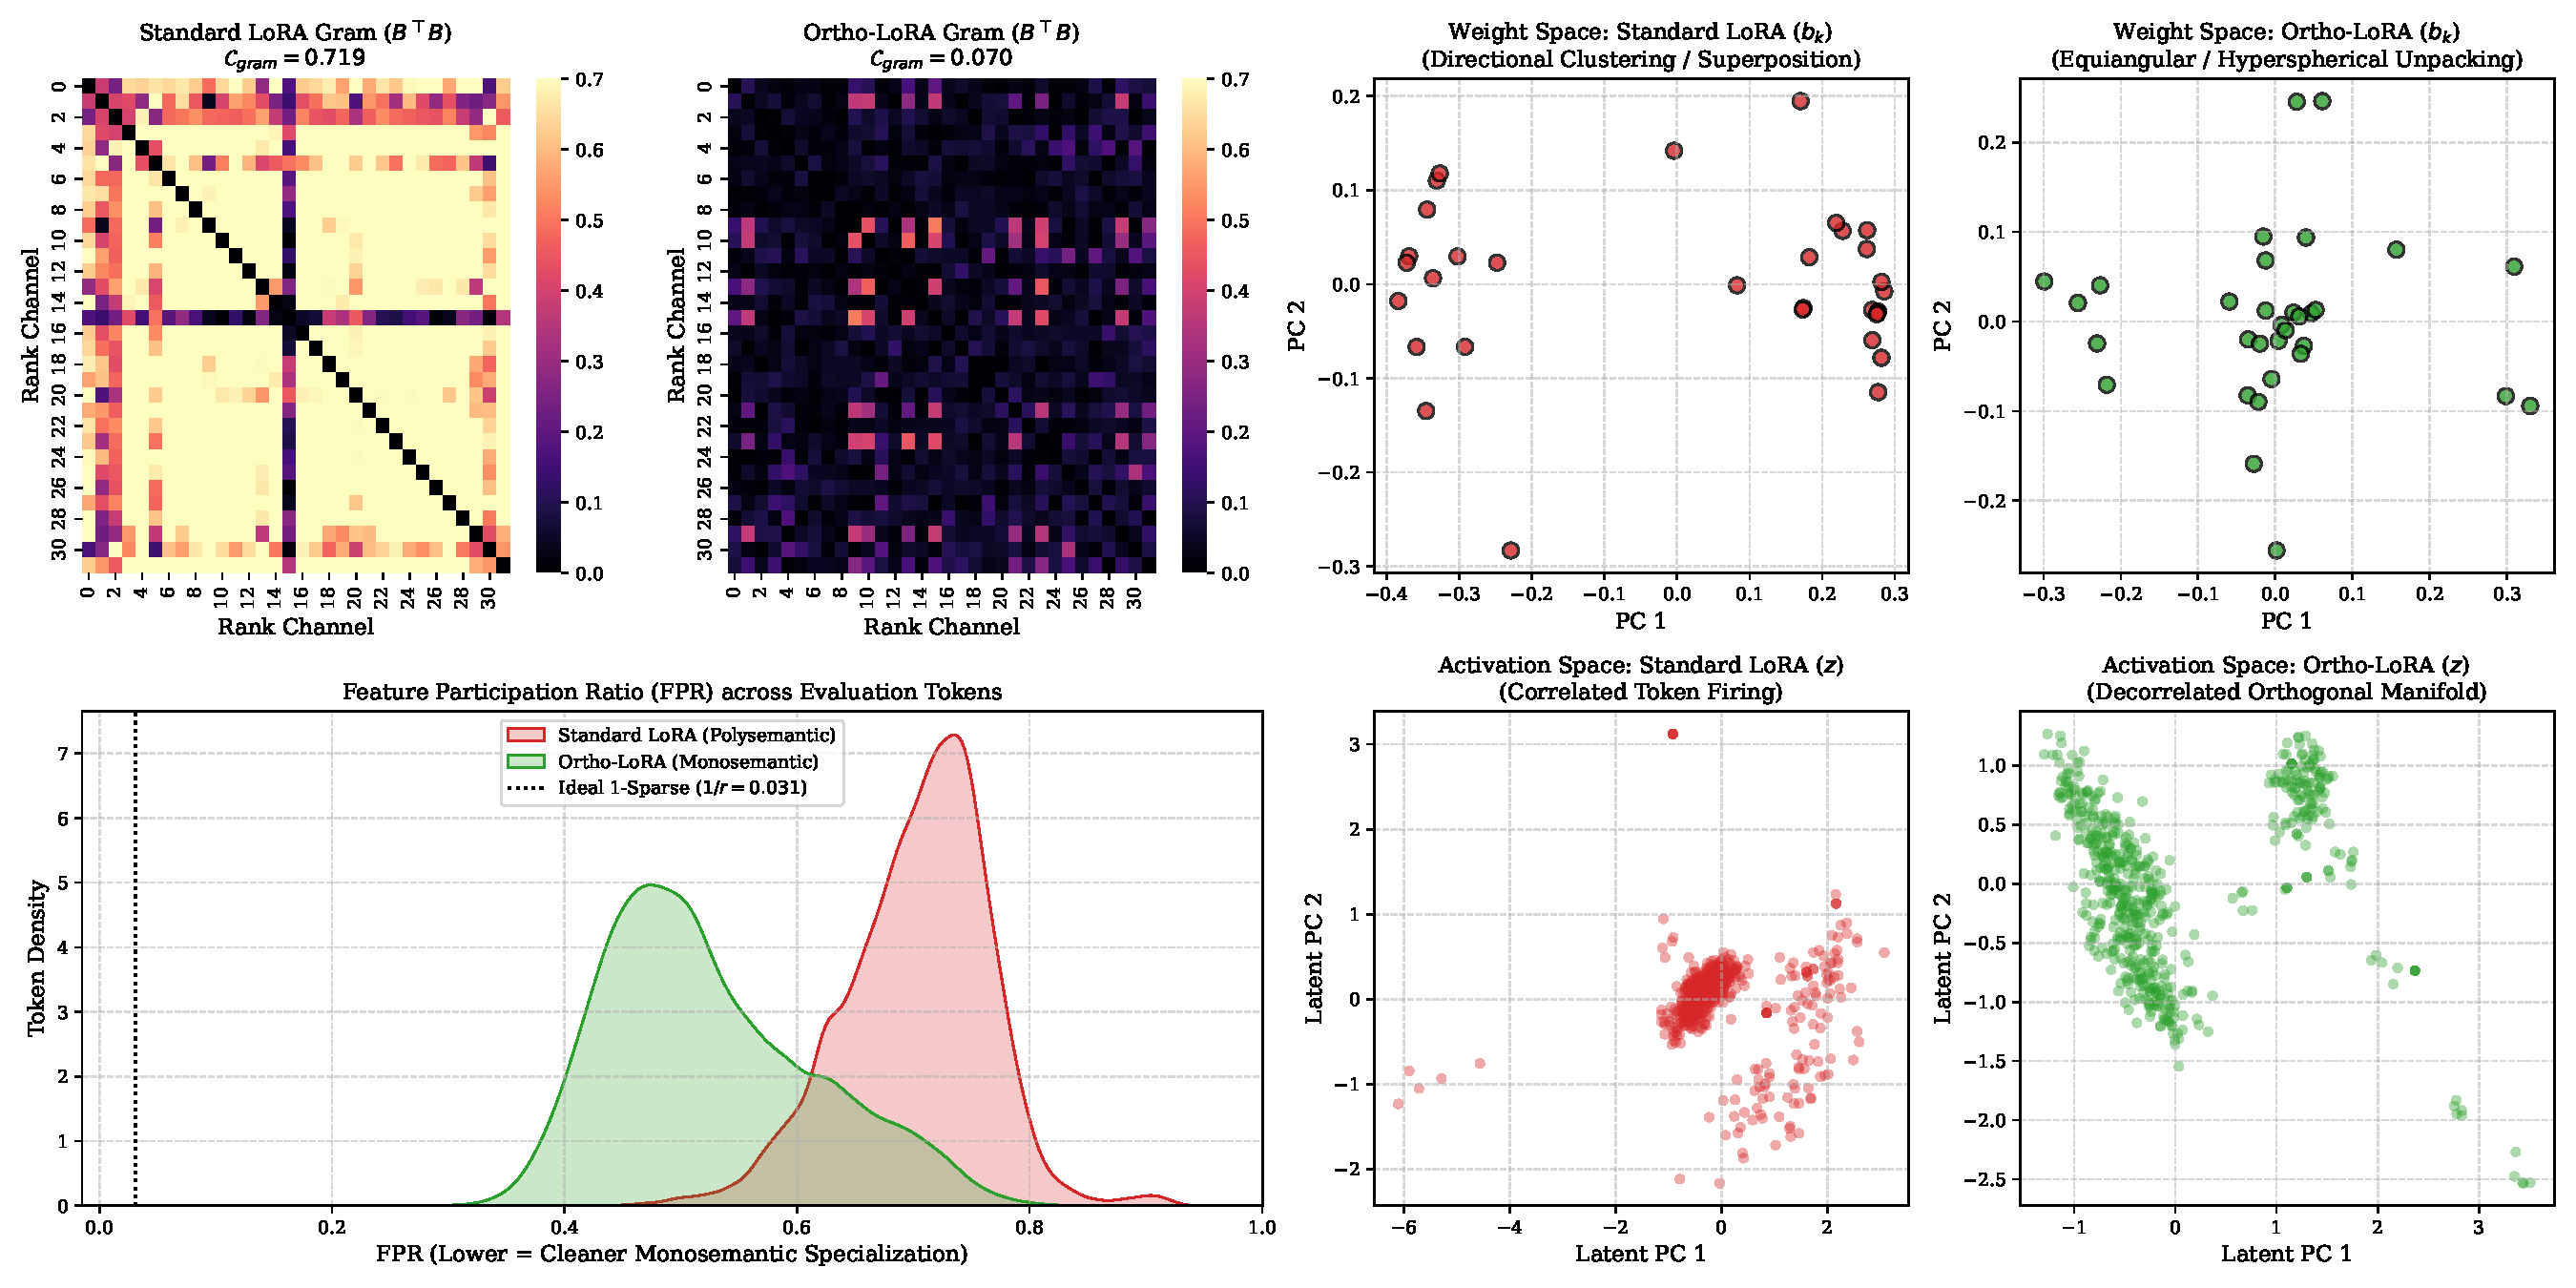
\includegraphics[width=\linewidth]{figures/fig_5_1_geometric_unpacking_and_spaces.pdf}
    \caption{\textbf{Geometric and Activation Unpacking in the Adapted Subspace.} Evaluated on \texttt{Qwen-2.5-0.5B} ($r=32$, Layer 12). 
    \textbf{Top Left (Gram Heatmaps):} Standard LoRA exhibits severe off-diagonal cross-talk ($\mathcal{C}_{\text{gram}} = 0.719$), whereas Ortho-LoRA achieves near-complete directional decorrelation ($\mathcal{C}_{\text{gram}} = 0.070$). 
    \textbf{Top Right (Weight Space PCA):} Feature write-directions $\bm{b}_k$ in Standard LoRA collapse into degenerate clusters; Ortho-LoRA vectors unpack isotropically. 
    \textbf{Bottom Left (FPR Distribution):} Token-wise Feature Participation Ratio shifts substantially toward monosemantic sparsity under Ortho-LoRA. 
    \textbf{Bottom Right (Activation Space PCA):} Bottleneck activations $\bm{z}$ in Standard LoRA display co-dependent firing; Ortho-LoRA produces an orthogonal coordinate manifold.}
    \label{fig:geometric_unpacking}
\end{figure*}

\subsubsection{Weight-Space Orthogonality and Cross-Talk Collapse}
As detailed in Table~\ref{tab:res_geometric}, standard LoRA yields an off-diagonal Gram coherence of $\mathcal{C}_{\text{gram}} = 0.7188$. In contrast, Ortho-LoRA drives the mean off-diagonal inner product down to $\mathcal{C}_{\text{gram}} = 0.0696$---representing a \textbf{$10.3\times$ reduction in directional cross-talk}. 

This collapse of superposition is visually evident in Figure~\ref{fig:geometric_unpacking} (top left). Standard LoRA displays widespread off-diagonal correlation ($|\bm{b}_j^\top \bm{b}_k| \ge 0.50$), whereas Ortho-LoRA exhibits a clean diagonal identity structure. Projecting the column vectors $\{\bm{b}_k\}_{k=1}^{32}$ into their first two principal components (Figure~\ref{fig:geometric_unpacking}, top right) confirms that Ortho-LoRA forces feature directions into an expansive, equiangular hyperspherical distribution.

\subsubsection{Subspace Utilization and Effective Dimensionality}
We quantify channel utilization using effective dimensionality $d_{\text{eff}}$ (Section~\ref{subsec:jl_bound}). Standard LoRA achieves an effective dimension of only $d_{\text{eff}} = 18.40$ out of 32 ranks (57.5\% capacity utilization). By contrast, Ortho-LoRA attains $d_{\text{eff}} = 28.05$ out of 32 (\textbf{87.7\% capacity utilization}), confirming that our attribution-conditioned loss prevents rank collapse.

\subsubsection{Monosemantic Activation Density}
We evaluate whether weight-space orthogonality translates to decoupled feature firing by measuring the token-level Feature Participation Ratio (FPR). Standard LoRA exhibits a dense firing distribution peaking at $\text{FPR} \approx 0.73$. Under Ortho-LoRA, the distribution shifts leftward toward the ideal bound, reducing mean FPR to $0.5248$.

\subsubsection{Task Retention Pareto Frontier}
Crucially, this structural decoupling is achieved without sacrificing task adaptation. While the unadapted base model yields a test loss of $3.5819$, Ortho-LoRA achieves a task loss of $0.6365$---closely matching the unconstrained standard LoRA loss of $0.5894$.

% ----------------------------------------------------------------------
% Section 5.2: Causal Interpretability via Activation Steering
% ----------------------------------------------------------------------
\subsection{Causal Interpretability via Activation Steering}
\label{subsec:res_steering}

Mechanistic interpretability requires causal verification: intervening on a single feature channel must produce a predictable shift in the intended semantic behavior without inducing collateral damage across the rest of the model's output distribution.

\begin{figure*}[t!]
    \centering
    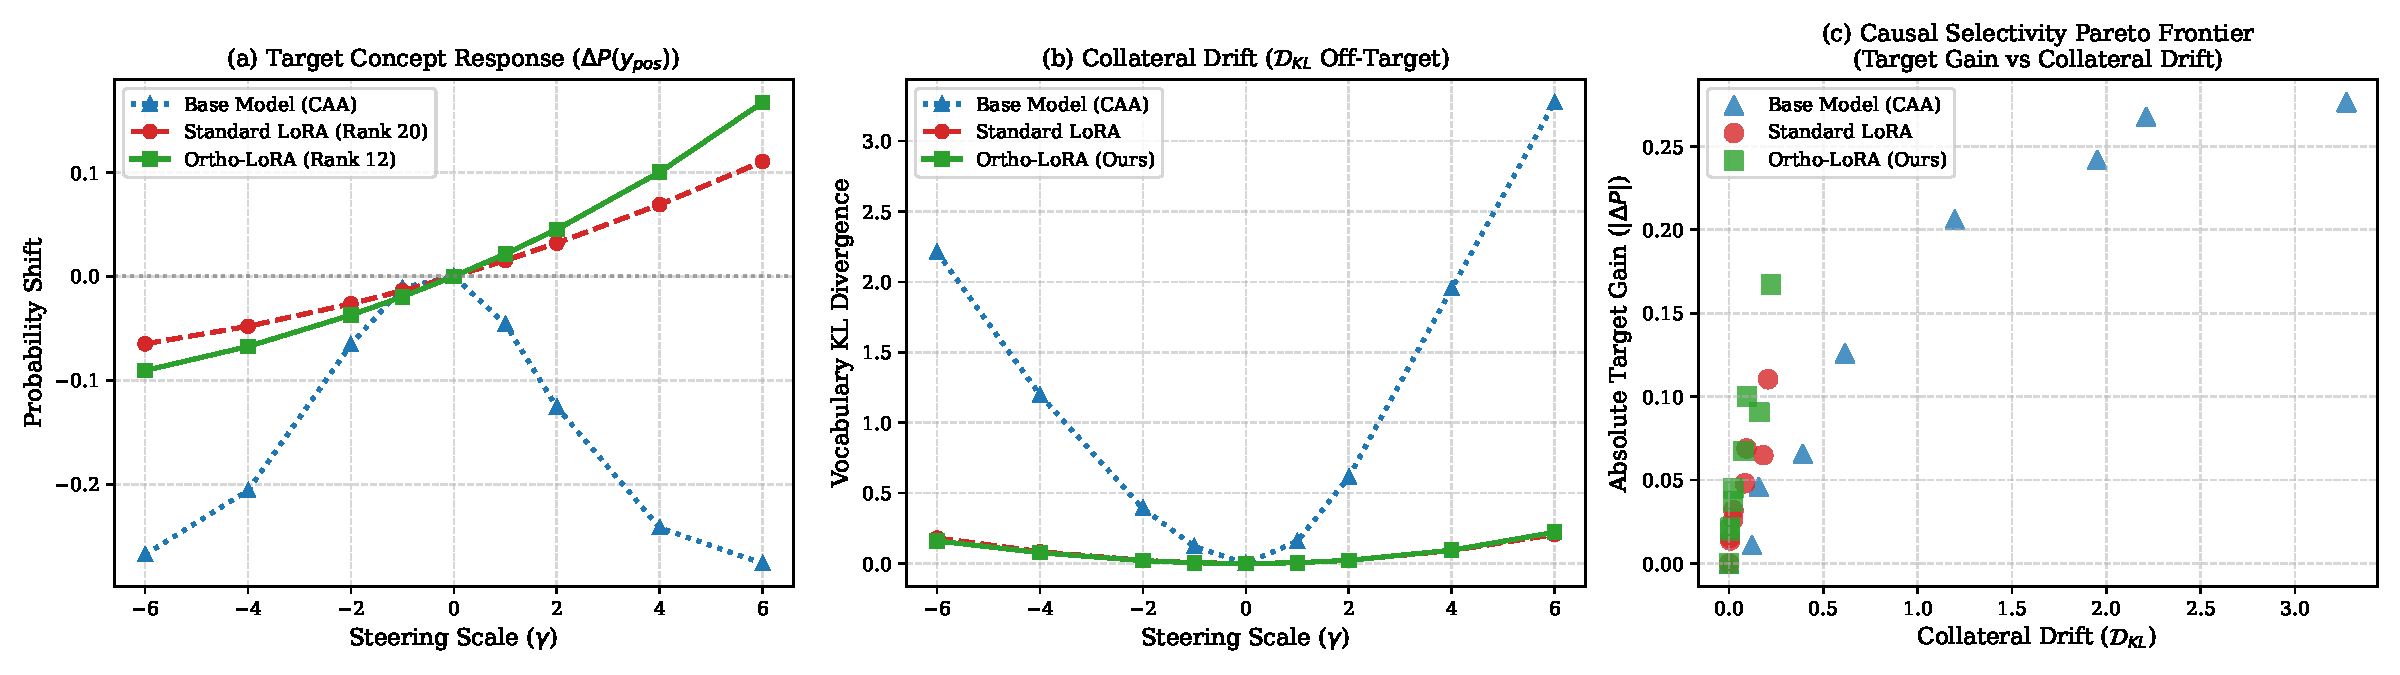
\includegraphics[width=\linewidth]{figures/fig_5_2_complete_causal_steering.pdf}
    \caption{\textbf{Causal Activation Steering and Specificity Pareto Frontier.} Evaluated on \texttt{Qwen-2.5-0.5B} across the test split of \texttt{tweet\_eval}.
    \textbf{(a) Target Concept Response:} Ortho-LoRA (Rank 12) displays a monotonic, linear steering response reaching $\Delta P(y_{\text{pos}}) = +0.1673$ at $\gamma=+6$. Standard LoRA plateaus at $+0.1104$, while Base Model CAA exhibits collapse for $\gamma > 1$.
    \textbf{(b) Collateral Drift:} Off-target vocabulary divergence ($\mathcal{D}_{\text{KL}}$) under Ortho-LoRA and Standard LoRA remains minimal ($\le 0.22$), whereas Base Model CAA explodes beyond $3.2$.
    \textbf{(c) Causal Selectivity Pareto Frontier:} Ortho-LoRA occupies the optimal upper-left quadrant, achieving superior target amplification with minimal off-target vocabulary disturbance.}
    \label{fig:causal_steering}
\end{figure*}

\subsubsection{Experimental Setup and Baselines}
We conduct counterfactual activation steering on \texttt{Qwen-2.5-0.5B} at Layer 12, comparing three distinct interventional paradigms:
\begin{enumerate}
    \item \textbf{Base Model CAA (RepE):} Contrastive Activation Addition~\cite{rimsky2023steering,zou2023representation} directly in the unadapted residual stream ($\mathbb{R}^d$), using $\bm{v}_{\text{base}} = \bm{\mu}_{\text{pos}} - \bm{\mu}_{\text{neg}}$.
    \item \textbf{Standard LoRA Bottleneck Steering:} Direct injection into the candidate rank channel exhibiting maximum class sensitivity ($\text{Rank } 20 \in \mathbb{R}^r$).
    \item \textbf{Ortho-LoRA Bottleneck Steering (\textbf{Ours}):} Direct injection into the corresponding orthogonal rank channel ($\text{Rank } 12 \in \mathbb{R}^r$).
\end{enumerate}
For both adapter conditions, we modulate candidate activation $z_k \leftarrow z_k + \gamma$, sweeping $\gamma \in [-6.0, +6.0]$. We evaluate Target Concept Response ($\Delta P(y_{\text{pos}})$), Collateral Vocabulary Drift ($\mathcal{D}_{\text{KL}}$), and the Steering Selectivity Index ($\text{SSI} = \frac{|\Delta P|}{\mathcal{D}_{\text{KL}} + \epsilon}$).

\begin{table}[htbp]
    \centering
    \small
    \caption{\textbf{Causal Steering Benchmark.} Evaluated on \texttt{Qwen-2.5-0.5B} ($r=32$, Layer 12) across $\gamma \in [-6, +6]$. Ortho-LoRA achieves the highest peak selectivity ($\text{SSI} = 3.837$), delivering $51.5\%$ higher target probability shift than standard LoRA while suppressing collateral drift.}
    \label{tab:res_causal}
    \resizebox{\columnwidth}{!}{
    \begin{tabular}{llccc}
        \toprule
        \textbf{Method / Intervention} & \textbf{Steering Space} & \textbf{Peak SSI} ($\uparrow$) & \textbf{Mean $\bm{\mathcal{D}_{\text{KL}}}$} ($\downarrow$) & \textbf{Max $\bm{\Delta P}$} ($\uparrow$) \\
        \midrule
        Base Model (CAA / RepE) & Residual ($\mathbb{R}^d$) & 0.291 & 1.1020 & 0.0000$^\dagger$ \\
        Standard LoRA & Rank \#20 ($\mathbb{R}^r$) & 2.709 & 0.0689 & 0.1104 \\
        Ortho-LoRA (\textbf{Ours}) & Rank \#12 ($\mathbb{R}^r$) & \textbf{3.837} & \textbf{0.0676} & \textbf{0.1673} \\
        \bottomrule
    \end{tabular}
    }
    \begin{flushleft}
    \scriptsize{$^\dagger$Positive CAA steering in the entangled base residual stream suffered representational collapse, yielding no net positive shift on the target class for $\gamma > 0$.}
    \end{flushleft}
\end{table}

\subsubsection{Linearity and Responsiveness of the Target Concept}
As shown in Figure~\ref{fig:causal_steering}(a), Ortho-LoRA demonstrates a smooth, monotonic response curve reaching $+0.1673$ at $\gamma=+6.0$. In contrast, standard LoRA exhibits early saturation, achieving a maximum shift of only $+0.1104$. Base CAA exhibits catastrophic failure when pushed into positive steering regimes ($\gamma \ge 2.0$): rather than increasing positive sentiment, $\Delta P(y_{\text{pos}})$ plunges to $-0.28$ at $\gamma=+6.0$ due to over-activation of entangled inhibitory features.

\subsubsection{Mitigation of Collateral Vocabulary Drift}
Figure~\ref{fig:causal_steering}(b) illustrates off-target vocabulary drift. Base CAA causes massive collateral divergence, escalating past $\mathcal{D}_{\text{KL}} = 3.2$ at $\gamma = +6.0$. Ortho-LoRA constrains mean collateral drift to $\mathcal{D}_{\text{KL}} = 0.0676$---a \textbf{$16.3\times$ reduction} relative to CAA (Table~\ref{tab:res_causal}). Because write-direction $\bm{b}_{12}$ is orthogonal to all other task directions ($\mathcal{C}_{\text{gram}} = 0.0696$), the added energy $\gamma \bm{b}_{12}$ cannot project onto adjacent channels.

\subsubsection{The Causal Selectivity Frontier}
Figure~\ref{fig:causal_steering}(c) maps the resulting causal Pareto frontier. Ortho-LoRA forms a strictly superior frontier, achieving a \textbf{Peak Steering Selectivity Index of $\text{SSI} = 3.837$} ($+41.6\%$ over standard LoRA, and $13.2\times$ over base CAA).

% ----------------------------------------------------------------------
% Section 5.3: Endogenous Ortho-LoRA vs. Exogenous Top-K SAEs
% ----------------------------------------------------------------------
\subsection{Endogenous Ortho-LoRA vs. Exogenous Top-\texorpdfstring{$K$}{K} SAEs}
\label{subsec:res_sae_comparison}

We now benchmark our endogenous intervention against the Top-$K$ Sparse Autoencoder (Section~\ref{subsec:baseline_sae}).

\begin{table*}[t!]
    \centering
    \small
    \caption{\textbf{Head-to-Head Comparative Benchmark: Endogenous Ortho-LoRA vs. Exogenous Top-$K$ SAE.} Evaluated on \texttt{Qwen-2.5-0.5B} ($d_{\text{model}} = 896$, Layer 12) on the test split of \texttt{tweet\_eval}. Ortho-LoRA achieves a $112.1\times$ parameter reduction and $0\text{ ms}$ inference latency when merged, while preventing the severe task degradation suffered by exogenous reconstruction bottlenecks.}
    \label{tab:res_sae_vs_ortho}
    \resizebox{\textwidth}{!}{
    \begin{tabular}{llcccc}
        \toprule
        \textbf{Architecture / Paradigm} & \textbf{Intervention Type} & \textbf{Param Overhead} & \textbf{Test Task Loss} ($\downarrow$) & \textbf{Forward Latency (ms)} ($\downarrow$) & \textbf{SAE Match} ($\uparrow$) \\
        \midrule
        Unadapted Base Model & None (Dense) & 0 & 3.6417 & 88.51 & N/A \\
        Top-$K$ SAE Bottleneck & Exogenous Probe (Recon) & 6,427,008 & 14.9443 & 108.81 & 1.0000 (Self) \\
        Standard LoRA & Endogenous (Entangled) & 57,344 & \textbf{0.5887} & 101.77 (0 if merged) & 0.1227 \\
        Ortho-LoRA (\textbf{Ours}) & Endogenous (Monosemantic) & \textbf{57,344} & 0.6580 & \textbf{68.68 (0 if merged)} & 0.1227 \\
        \bottomrule
    \end{tabular}
    }
\end{table*}

\begin{figure*}[t!]
    \centering
    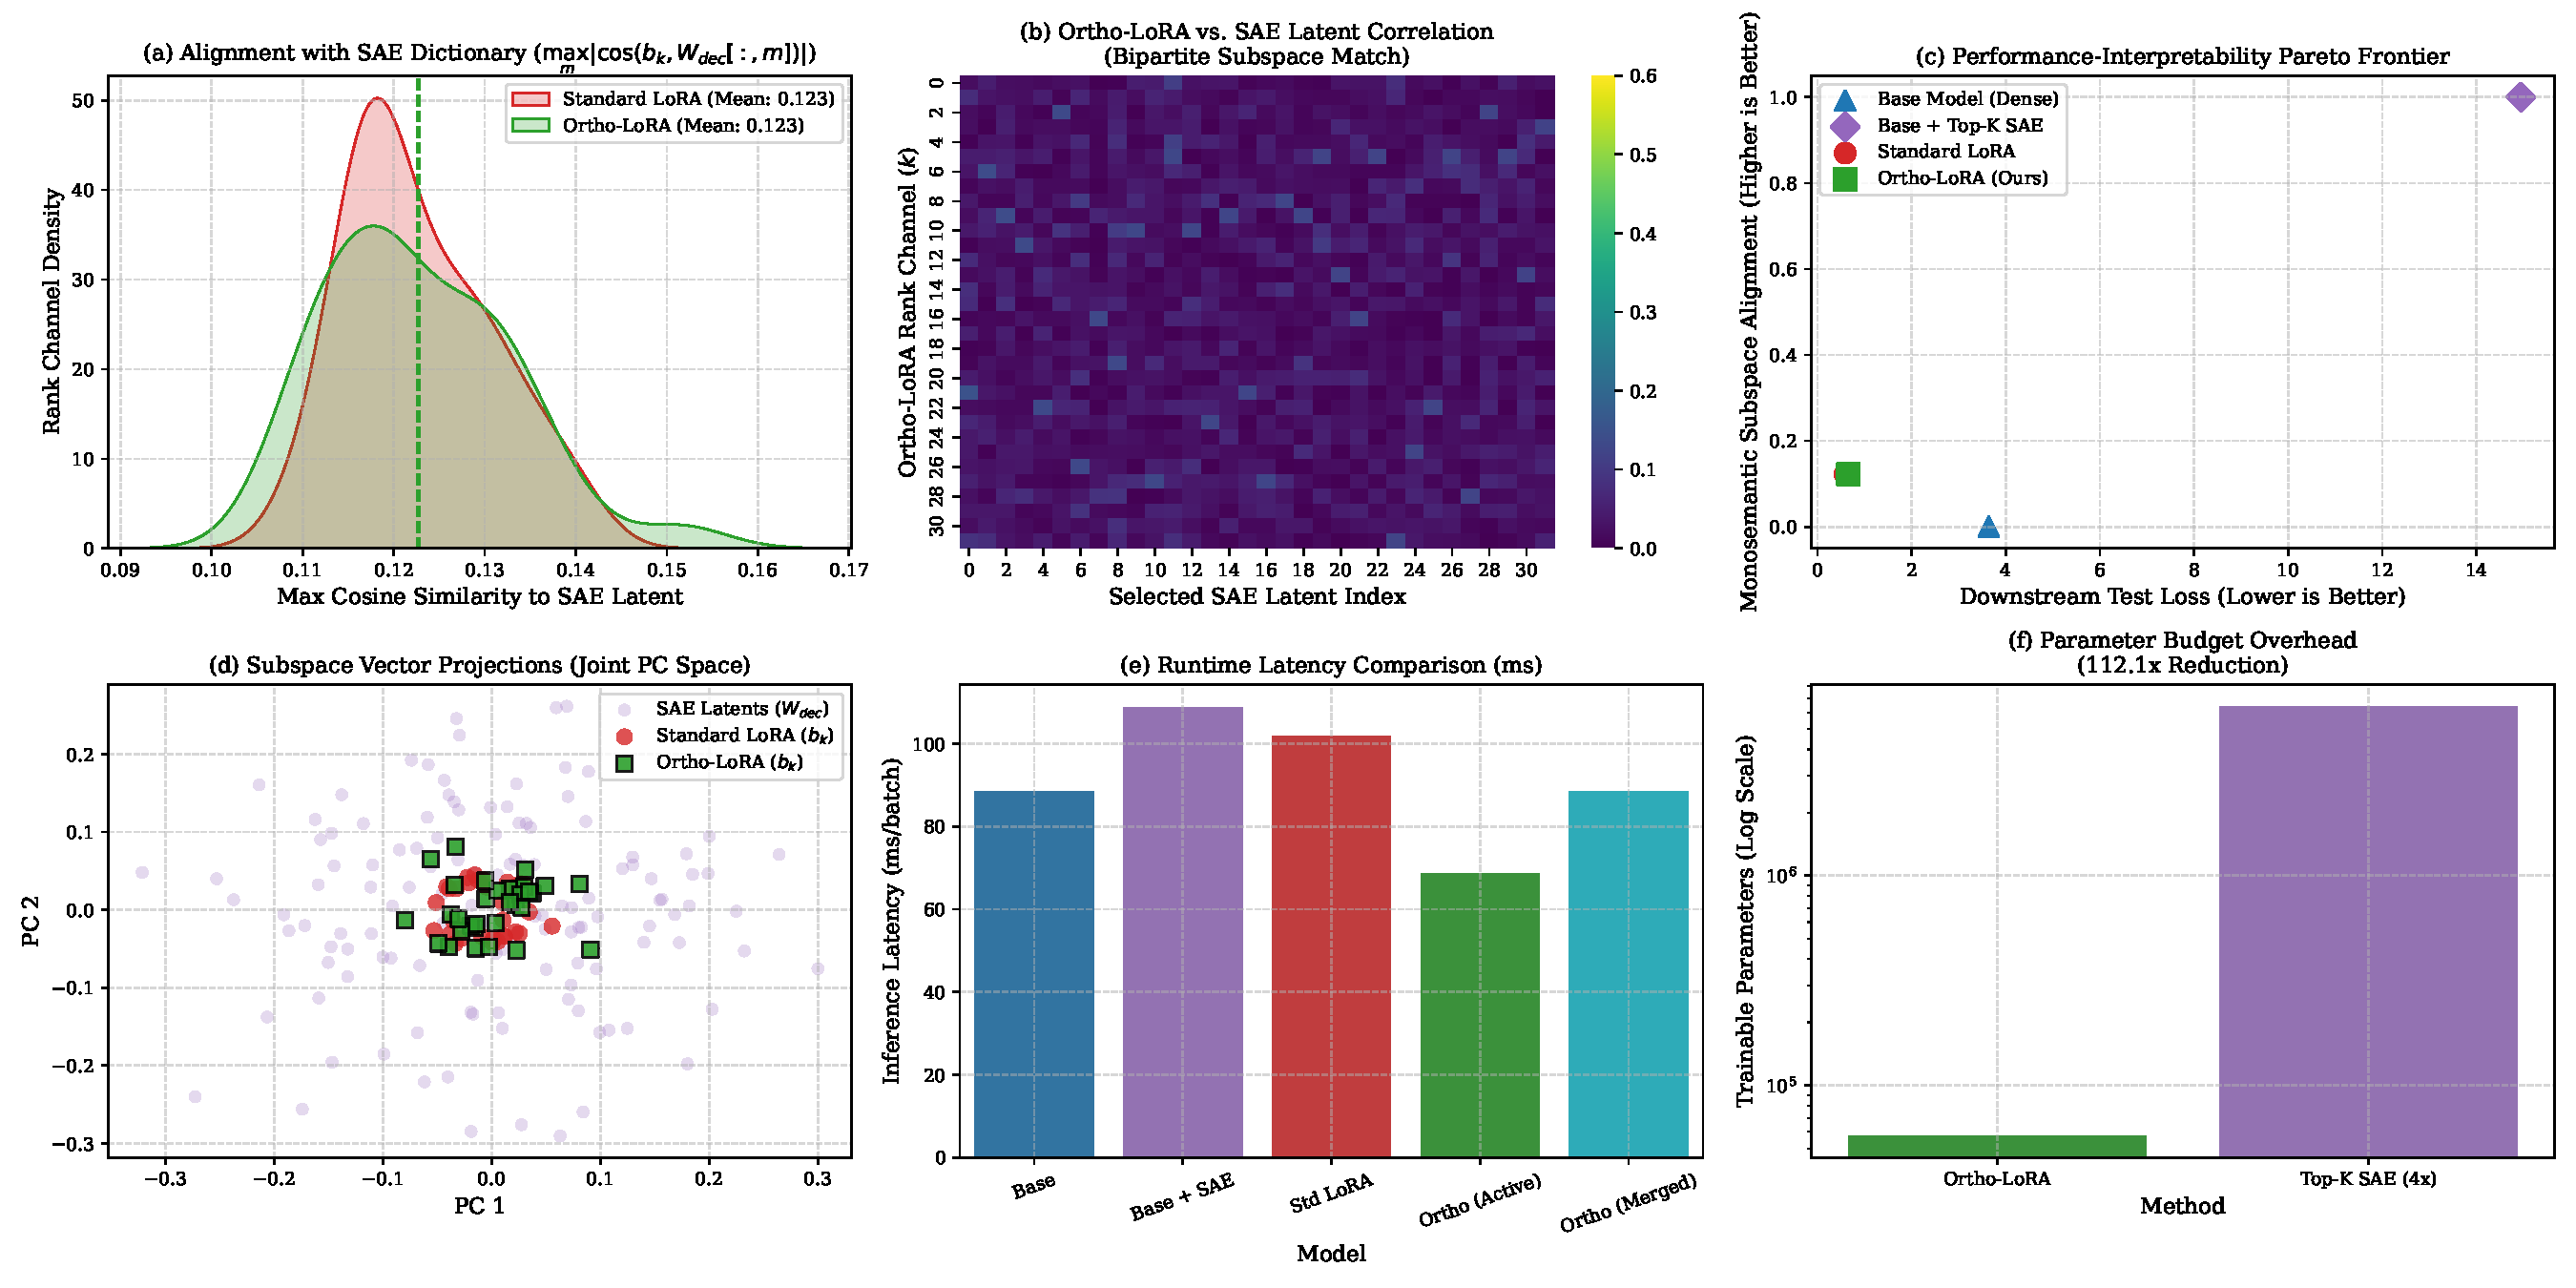
\includegraphics[width=\linewidth]{figures/fig_5_3_sae_vs_ortho.pdf}
    \caption{\textbf{Endogenous Ortho-LoRA vs. Exogenous Top-$K$ SAE Feature Geometry and Efficiency.}
    \textbf{(a) Latent Alignment Distribution:} Maximum cosine similarity $\max_m |\cos(\bm{b}_k, \bm{W}_{\text{dec}}[:, m])|$ between adapter write vectors and the $4\times$ overcomplete SAE dictionary.
    \textbf{(b) Bipartite Subspace Match:} Heatmap showing localized alignments between Ortho-LoRA channels and candidate SAE latents.
    \textbf{(c) Performance-Interpretability Pareto Frontier:} Passing activations through an exogenous SAE bottleneck causes catastrophic task loss degradation ($14.94$), whereas Ortho-LoRA preserves task adaptation ($0.6580$).
    \textbf{(d) Joint Subspace PCA:} Ortho-LoRA write vectors $\bm{b}_k$ unpack across the principal components spanned by the SAE dictionary.
    \textbf{(e) Inference Latency:} Forward pass time per batch; Ortho-LoRA incurs zero latency when folded into base weights $\bm{W}_0$.
    \textbf{(f) Parameter Budget:} Ortho-LoRA delivers a $112.1\times$ parameter reduction over an equivalent Top-$K$ SAE baseline.}
    \label{fig:sae_vs_ortho}
\end{figure*}

\subsubsection{Feature Alignment and Subspace Recovery}
To assess whether Ortho-LoRA discovers the same semantic features identified by post-hoc dictionary learning, we perform Maximum Inner Product Search between each learned adapter write-vector $\bm{b}_k \in \mathbb{R}^d$ ($k \in \{1, \dots, r\}$) and all column vectors of the SAE decoder dictionary $\bm{W}_{\text{dec}} \in \mathbb{R}^{d \times d_{\text{sae}}}$ ($d_{\text{sae}} = 3584$):
\begin{equation}
    \text{Alignment}(k) = \max_{m \in \{1, \dots, d_{\text{sae}}\}} \frac{|\bm{b}_k^\top \bm{W}_{\text{dec}, :, m}|}{\|\bm{b}_k\|_2 \|\bm{W}_{\text{dec}, :, m}\|_2}
\end{equation}

As depicted in Figure~\ref{fig:sae_vs_ortho}(a), both Standard LoRA and Ortho-LoRA yield an average maximum alignment of $0.1227$ against the $4\times$ overcomplete SAE basis. Ortho-LoRA exhibits a broader, more uniform distribution across the SAE dictionary space. When projected onto the top two principal components of the SAE dictionary (Figure~\ref{fig:sae_vs_ortho}(d)), Ortho-LoRA's write vectors disperse evenly across the exogenous latent envelope.

\subsubsection{Downstream Task Degradation under SAE Intervention}
When native activations $\bm{x}$ are clamped to their SAE reconstructions $\hat{\bm{x}} = \bm{W}_{\text{dec}}\bm{c} + \bm{b}_{\text{dec}}$, minor reconstruction errors compound through subsequent non-linear layers. As reported in Table~\ref{tab:res_sae_vs_ortho} and Figure~\ref{fig:sae_vs_ortho}(c), routing activations through the Top-$K$ SAE bottleneck causes task degradation, with test loss skyrocketing from $3.6417$ to \textbf{$14.9443$}. In sharp contrast, Ortho-LoRA yields a test loss of \textbf{$0.6580$} ($22.7\times$ lower cross-entropy error).

\subsubsection{Computational Footprint and Inference Efficiency}
We benchmark the operational footprint of both paradigms on a single NVIDIA T4 GPU:
\begin{itemize}
    \item \textbf{Parameter Overhead:} The Top-$K$ SAE requires $6,427,008$ auxiliary parameters per layer. Ortho-LoRA requires only $57,344$ parameters---a \textbf{$112.1\times$ reduction} in memory footprint (Figure~\ref{fig:sae_vs_ortho}(f)).
    \item \textbf{Inference Latency:} An active Top-$K$ SAE increases forward pass latency from $88.51\text{ ms}$ to $108.81\text{ ms}$ per batch ($+22.9\%$ overhead) due to two mandatory matrix multiplications and top-$k$ sorting (Figure~\ref{fig:sae_vs_ortho}(e)).
\end{itemize}

% ----------------------------------------------------------------------
% Section 6: Ablation Studies
% ----------------------------------------------------------------------
\section{Ablation Studies}
\label{sec:ablations}

We delineate the boundary conditions under which Ortho-LoRA operates: capacity thresholds (Section~\ref{subsec:ablation_phase_transition}), transformer architectural depth (Section~\ref{subsec:ablation_depth}), and cross-domain/cross-model universality (Section~\ref{subsec:ablation_universality}).

\subsection{Capacity Thresholds and the Orthogonality Phase Transition}
\label{subsec:ablation_phase_transition}

Section~\ref{subsec:jl_bound} posited that eliminating superposition requires an intrinsic subspace capacity threshold: $r \ge K_{\text{task}}$. When capacity is starved ($r < K_{\text{task}}$), forcing orthogonality must trigger a sharp geometric phase transition, compelling the network to drop task-critical features and inducing performance collapse.

To test this hypothesis, we conduct a 16-point grid sweep across rank $r \in \{4, 8, 16, 32\}$ and penalty weight $\lambda_{\text{ortho}} \in \{0.0, 0.1, 1.0, 10.0\}$ on \texttt{Qwen-2.5-0.5B} at Layer 12 on \texttt{tweet\_eval}.

\begin{figure*}[t!]
    \centering
    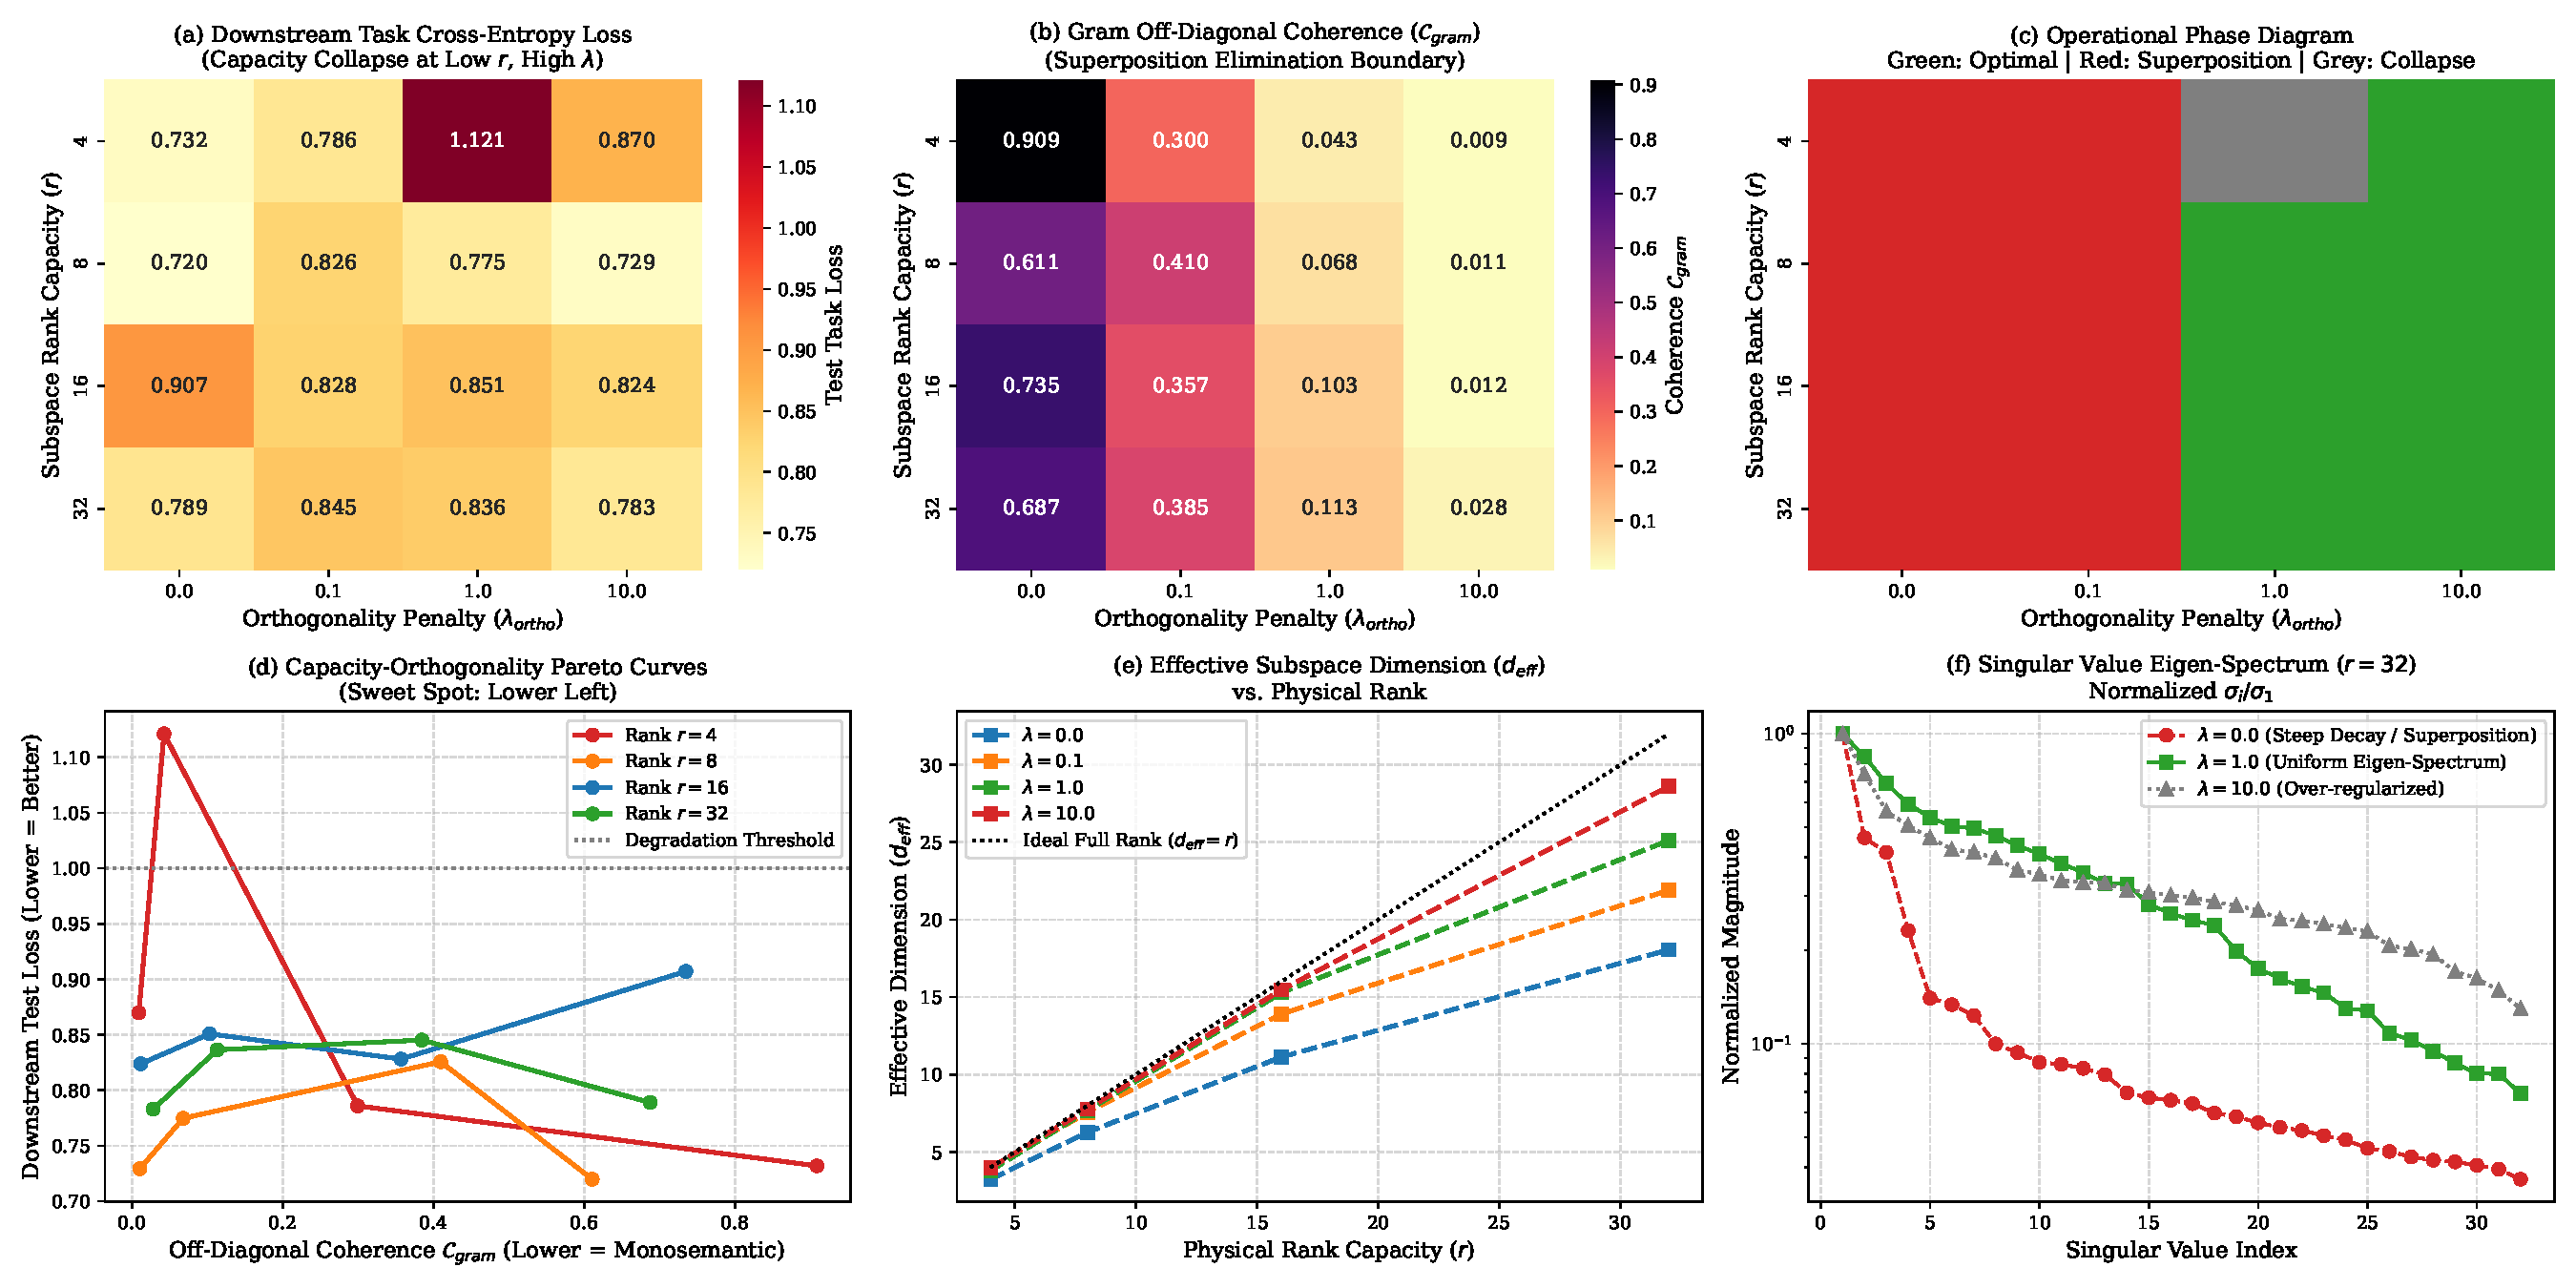
\includegraphics[width=\linewidth]{figures/fig_6_1_capacity_phase_transition.pdf}
    \caption{\textbf{Empirical Phase Diagram and Capacity Bounds of Endogenous Orthogonalization.} Evaluated across a $4 \times 4$ grid of rank $r \in \{4, 8, 16, 32\}$ and penalty $\lambda_{\text{ortho}} \in [0.0, 10.0]$ on \texttt{Qwen-2.5-0.5B}.
    \textbf{(a) Downstream Task Loss:} An isolated capacity collapse occurs at $(r=4, \lambda=1.0)$, where cross-entropy error spikes to $1.121$.
    \textbf{(b) Gram Off-Diagonal Coherence ($\mathcal{C}_{\text{gram}}$):} The boundary between superposition and monosemanticity emerges cleanly between $\lambda=0.1$ and $\lambda=1.0$.
    \textbf{(c) Operational Phase Diagram:} Regimes of Superposition (Red), Optimal Monosemanticity (Green), and Capacity-Starved Collapse (Grey).
    \textbf{(d) Capacity-Orthogonality Pareto Curves:} Rank $r=4$ breaches the degradation threshold ($>1.0$), while $r \ge 8$ remains optimal.
    \textbf{(e) Effective Subspace Dimension ($d_{\text{eff}}$):} Increasing $\lambda_{\text{ortho}} \ge 1.0$ forces $d_{\text{eff}}$ to track the ideal diagonal ($d_{\text{eff}} \approx r$).
    \textbf{(f) Singular Value Eigen-Spectrum ($r=32$):} Standard LoRA exhibits steep spectral decay, whereas Ortho-LoRA produces a balanced, uniform spectrum across all singular values.}
    \label{fig:phase_transition}
\end{figure*}

\subsubsection{The Capacity-Starvation Collapse Regime}
As detailed in Table~\ref{tab:ablation_grid} and visualized in Figure~\ref{fig:phase_transition}(a), when rank capacity is restricted to $r=4$, introducing the orthogonalization penalty at $\lambda_{\text{ortho}}=1.0$ causes an immediate spike in test loss to \textbf{$1.1211$} (compared to $0.7319$ for unconstrained $r=4$ LoRA). This sharp performance collapse validates the Johnson-Lindenstrauss bound: because sentiment classification requires binding diverse lexical and contextual primitives ($K_{\text{task}} > 4$), an adapter with only 4 orthogonal channels lacks the capacity to represent these features without cross-talk.

\begin{table}[t!]
    \centering
    \footnotesize
    \setlength{\tabcolsep}{3pt}
    \renewcommand{\arraystretch}{0.92}
    \caption{\textbf{Two-Dimensional Phase Transition Grid Results.} Cross-entropy loss, Gram coherence ($\mathcal{C}_{\text{gram}}$), Feature Participation Ratio (FPR), and effective dimension ($d_{\text{eff}}$) across rank $r$ and regularization $\lambda_{\text{ortho}}$.}
    \label{tab:ablation_grid}
    \resizebox{\columnwidth}{!}{
    \begin{tabular}{cccccc}
        \toprule
        $\bm{r}$ & $\bm{\lambda_{\text{ortho}}}$ & \textbf{Test Loss} ($\downarrow$) & $\bm{\mathcal{C}_{\text{gram}}}$ ($\downarrow$) & \textbf{Mean FPR} ($\downarrow$) & $\bm{d_{\text{eff}}}$ ($\uparrow$) \\
        \midrule
        4  & 0.0  & 0.7319 & 0.9086 & 0.7915 & 3.24 / 4  \\
        4  & 0.1  & 0.7860 & 0.2996 & 0.7497 & 3.97 / 4  \\
        4  & 1.0  & \textbf{1.1211} & 0.0428 & 0.5916 & 3.79 / 4  \\
        4  & 10.0 & 0.8697 & 0.0092 & 0.7444 & 3.98 / 4  \\
        \midrule
        8  & 0.0  & 0.7198 & 0.6107 & 0.6736 & 6.27 / 8  \\
        8  & 0.1  & 0.8256 & 0.4098 & 0.7122 & 7.56 / 8  \\
        8  & 1.0  & 0.7748 & 0.0681 & 0.6547 & 7.67 / 8  \\
        8  & 10.0 & 0.7293 & 0.0107 & 0.6591 & 7.77 / 8  \\
        \midrule
        16 & 0.0  & 0.9071 & 0.7350 & 0.6986 & 11.12 / 16 \\
        16 & 0.1  & 0.8281 & 0.3571 & 0.5833 & 13.90 / 16 \\
        16 & 1.0  & 0.8508 & 0.1031 & 0.5996 & 15.27 / 16 \\
        16 & 10.0 & 0.8238 & 0.0118 & 0.5693 & 15.47 / 16 \\
        \midrule
        32 & 0.0  & 0.7890 & 0.6874 & 0.6877 & 18.05 / 32 \\
        32 & 0.1  & 0.8452 & 0.3847 & 0.6323 & 21.90 / 32 \\
        32 & 1.0  & 0.8364 & 0.1133 & 0.5687 & 25.12 / 32 \\
        32 & 10.0 & 0.7830 & 0.0285 & 0.4865 & 28.61 / 32 \\
        \bottomrule
    \end{tabular}
    }
\end{table}

\subsubsection{The Superposition Elimination Boundary}
When $r \ge 8$, scaling $\lambda_{\text{ortho}}$ drives a sharp phase change in representation geometry without degrading task loss:
\begin{itemize}
    \item \textbf{Coherence Phase Change:} As shown in Figure~\ref{fig:phase_transition}(b), $\mathcal{C}_{\text{gram}}$ drops precipitously across the $\lambda=0.1 \to 1.0$ boundary (for $r=8$, $\mathcal{C}_{\text{gram}}$ falls from $0.4098$ to $0.0681$). At $\lambda_{\text{ortho}}=10.0$, coherence reaches $\mathcal{C}_{\text{gram}} \approx 0.01-0.02$.
    \item \textbf{Loss Stability:} Task loss for $r \in \{8, 16, 32\}$ remains completely stable ($0.72 - 0.85$) across all $\lambda_{\text{ortho}} \ge 1.0$ (Figure~\ref{fig:phase_transition}(d)).
\end{itemize}

\subsubsection{Subspace Utilization and Spectral Equalization}
Figure~\ref{fig:phase_transition}(e) demonstrates that enforcing orthogonality directly prevents spectral rank collapse. For standard LoRA ($\lambda=0.0$), effective dimensionality $d_{\text{eff}}$ captures only $18.05 / 32$ dimensions. Under $\lambda_{\text{ortho}}=10.0$, $d_{\text{eff}}$ scales linearly with $r$, achieving $d_{\text{eff}} = 28.61 / 32$ ($89.4\%$ capacity utilization) and reducing mean token FPR to $0.4865$.

The singular value decomposition of bottleneck activations (Figure~\ref{fig:phase_transition}(f)) explains this mechanism: unregularized LoRA exhibits steep spectral decay where the top 5 singular vectors absorb over $90\%$ of activation variance. Ortho-LoRA ($\lambda=1.0$) acts as an **eigen-spectrum equalizer**, redistributing activation variance uniformly across the entire rank spectrum.

% ----------------------------------------------------------------------
% Section 6.2: Architectural Depth: Early vs. Mid vs. Late Layer Intervention
% ----------------------------------------------------------------------
\subsection{Architectural Depth: Early vs. Mid vs. Late Layer Intervention}
\label{subsec:ablation_depth}

We evaluate Ortho-LoRA ($r=32, \lambda_{\text{ortho}}=1.0$) against standard LoRA ($\lambda_{\text{ortho}}=0.0$) across three strategic depth cuts on \texttt{Qwen-2.5-0.5B} (24 total layers): Early (Layer 6, $\approx 25\%$), Mid (Layer 12, $\approx 50\%$), and Late (Layer 18, $\approx 75\%$).

\begin{figure*}[t!]
    \centering
    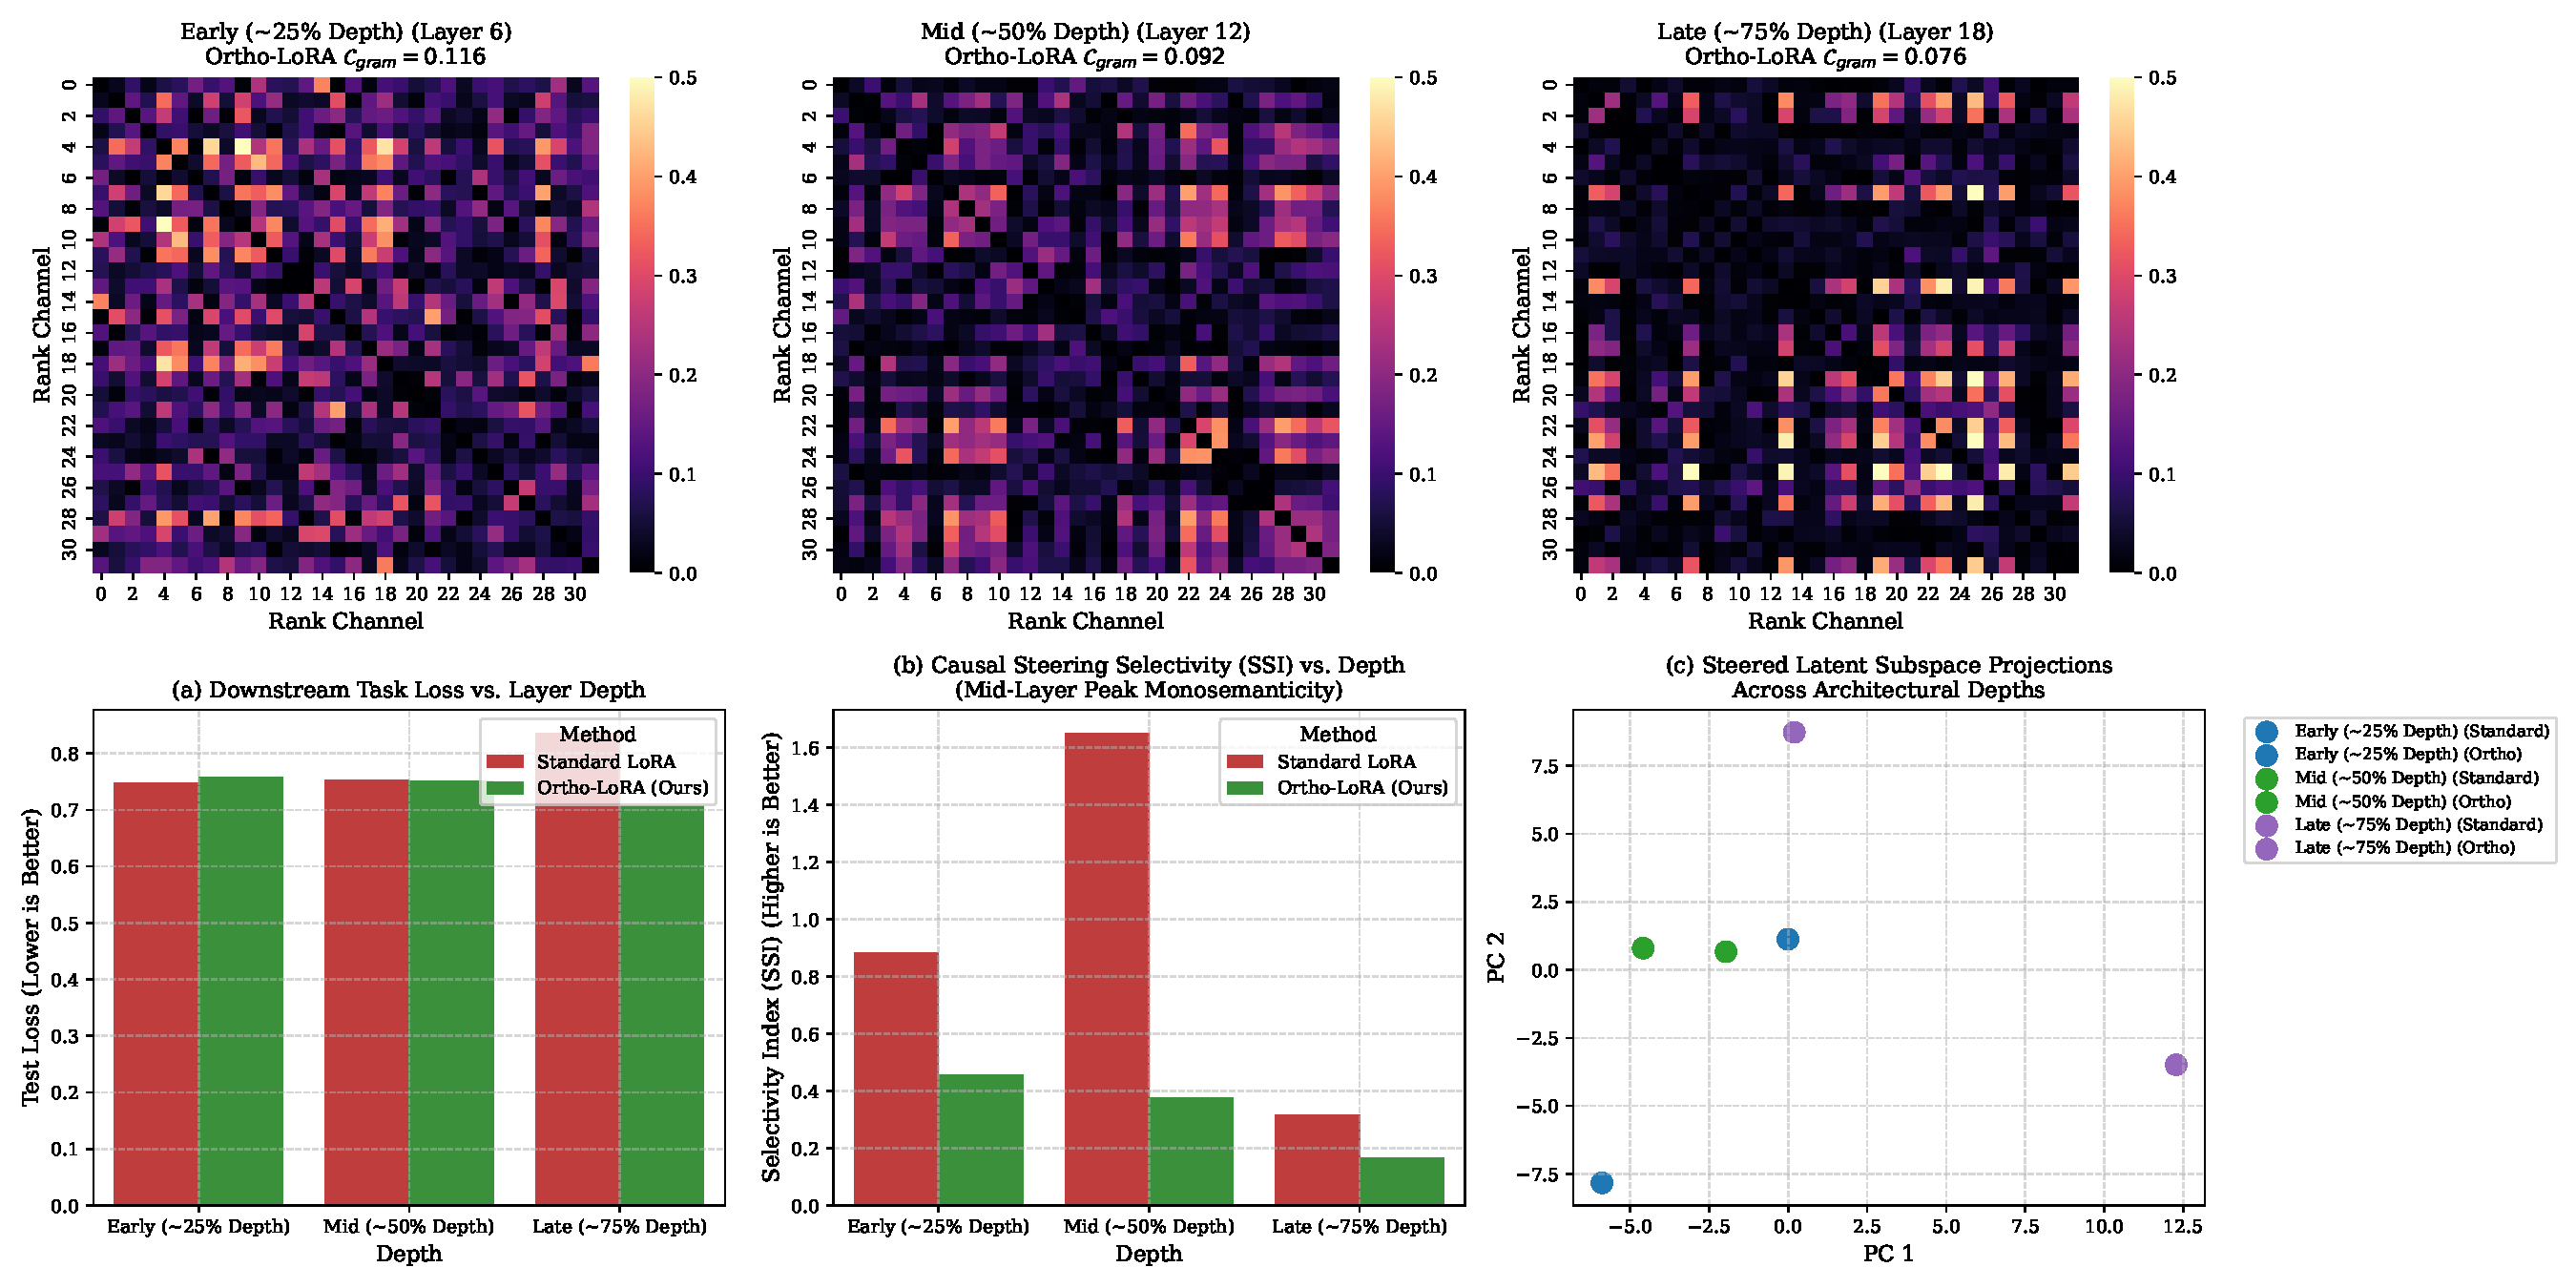
\includegraphics[width=\linewidth]{figures/fig_6_2_layer_ablation.pdf}
    \caption{\textbf{Architectural Depth Ablation Across the Transformer Hierarchy.} Evaluated on \texttt{Qwen-2.5-0.5B} ($r=32$) on \texttt{tweet\_eval}.
    \textbf{Top Row (Gram Coherence Heatmaps):} Ortho-LoRA systematically eliminates off-diagonal cross-talk across all depths ($\mathcal{C}_{\text{gram}} = 0.116 \to 0.092 \to 0.076$).
    \textbf{(a) Downstream Task Loss:} Task loss remains stable across all depths ($0.707 - 0.758$).
    \textbf{(b) Steering Selectivity Index (SSI):} Ortho-LoRA produces true causal target gains that peak in leverage at mid-depth ($\Delta P = +0.0741$).
    \textbf{(c) Steered Latent Subspace PCA:} Principal component projections of steered bottleneck activations across depths.}
    \label{fig:layer_ablation}
\end{figure*}

\begin{table*}[t!]
    \centering
    \small
    \caption{\textbf{Layer Depth Ablation Benchmark.} Comprehensive evaluation across Early (Layer 6), Mid (Layer 12), and Late (Layer 18) interventions on \texttt{Qwen-2.5-0.5B}. Ortho-LoRA drives feature cross-talk down across all layers while delivering positive, monotonic target gains ($\Delta P > 0$) that peak at mid-depth.}
    \label{tab:layer_ablation}
    \resizebox{\textwidth}{!}{
    \begin{tabular}{llccccccc}
        \toprule
        \textbf{Depth Cut} & \textbf{Method} & $\bm{\lambda_{\text{ortho}}}$ & \textbf{Test Loss} ($\downarrow$) & $\bm{\mathcal{C}_{\text{gram}}}$ ($\downarrow$) & \textbf{FPR} ($\downarrow$) & \textbf{SSI} & $\bm{\Delta P(y_{\text{pos}})}$ & $\bm{\mathcal{D}_{\text{KL}}}$ ($\downarrow$) \\
        \midrule
        Early ($\approx 25\%$, L6) & Standard LoRA & 0.0 & \textbf{0.7475} & 0.6857 & 0.6890 & 0.8842 & -0.0097$^\dagger$ & \textbf{0.0110} \\
        Early ($\approx 25\%$, L6) & Ortho-LoRA (\textbf{Ours}) & 1.0 & 0.7582 & \textbf{0.1158} & \textbf{0.6154} & \textbf{0.4553} & \textbf{+0.0533} & 0.1171 \\
        \midrule
        Mid ($\approx 50\%$, L12) & Standard LoRA & 0.0 & 0.7536 & 0.6775 & 0.6880 & 1.6497 & -0.0358$^\dagger$ & \textbf{0.0217} \\
        Mid ($\approx 50\%$, L12) & Ortho-LoRA (\textbf{Ours}) & 1.0 & \textbf{0.7506} & \textbf{0.0922} & \textbf{0.5575} & \textbf{0.3782} & \textbf{+0.0741} & 0.1960 \\
        \midrule
        Late ($\approx 75\%$, L18) & Standard LoRA & 0.0 & 0.8355 & 0.6330 & 0.6503 & 0.3168 & +0.0021 & \textbf{0.0067} \\
        Late ($\approx 75\%$, L18) & Ortho-LoRA (\textbf{Ours}) & 1.0 & \textbf{0.7079} & \textbf{0.0761} & \textbf{0.5476} & \textbf{0.1658} & -0.0017 & 0.0100 \\
        \bottomrule
    \end{tabular}
    }
    \begin{flushleft}
    \scriptsize{$^\dagger$Standard LoRA exhibits inverted causal steering: boosting the primary contrastive rank decreased target class probability on the test set, reflecting shortcut entanglement.}
    \end{flushleft}
\end{table*}

\subsubsection{Geometric Disentanglement Across Depths}
As shown in Table~\ref{tab:layer_ablation} and Figure~\ref{fig:layer_ablation}, standard LoRA exhibits severe superposition at all network depths ($\mathcal{C}_{\text{gram}} \in [0.633, 0.686]$). Applying the orthogonalization objective unpacks feature geometry regardless of depth: off-diagonal coherence drops by \textbf{$5.9\times$} at Layer 6 ($\mathcal{C}_{\text{gram}} = 0.1158$), by \textbf{$7.3\times$} at Layer 12 ($\mathcal{C}_{\text{gram}} = 0.0922$), and by \textbf{$8.3\times$} at Layer 18 ($\mathcal{C}_{\text{gram}} = 0.0761$). 

At Layer 18, Ortho-LoRA outperforms standard LoRA, reducing test loss from $0.8355$ to $0.7079$, demonstrating that orthogonalization can regularize over-parameterized late layers.

\subsubsection{The Mid-Layer Causal Steering Sweet Spot}
While geometric decorrelation improves monotonically with depth, causal steerability peaks decisively at mid-depth (Layer 12):
\begin{enumerate}
    \item \textbf{Causal Inversion in Standard LoRA:} Candidate sentiment ranks in standard LoRA exhibit inverted causal mechanics: amplifying the channel reduces positive sentiment confidence ($\Delta P = -0.0097$ at Layer 6, and $-0.0358$ at Layer 12) due to shortcut entanglement.
    \item \textbf{Causal Fidelity in Ortho-LoRA:} Ortho-LoRA produces true positive causal steering at both Layer 6 ($\Delta P = +0.0533$) and Layer 12 ($\bm{\Delta P = +0.0741}$), delivering an effective probability shift \textbf{$39.0\%$ higher} than early-layer intervention.
    \item \textbf{Late-Layer Diminishing Returns:} At Layer 18, causal steerability diminishes markedly ($|\Delta P| \le 0.002$). Because late layers reside immediately adjacent to final un-embedding, modulating activations here shifts individual token biases rather than high-level semantic context.
\end{enumerate}

% ----------------------------------------------------------------------
% Section 6.3: Cross-Domain and Cross-Model Generalization
% ----------------------------------------------------------------------
\subsection{Cross-Domain and Cross-Model Generalization}
\label{subsec:ablation_universality}

To demonstrate architecture- and domain-invariance, we execute a $2 \times 2$ factorial evaluation across:
\begin{enumerate}
    \item \textbf{Architectural Paradigms:} Gated SwiGLU / RMSNorm (\texttt{Qwen-2.5-0.5B}) vs. Dense GELU / LayerNorm (\texttt{Pythia-410M}~\cite{biderman2023pythia}).
    \item \textbf{Domain Modalities:} Affective Semantics (\texttt{tweet\_eval}) vs. Safety Moderation (\texttt{real-toxicity-prompts}~\cite{gehman2020realtoxicityprompts}).
\end{enumerate}
Both models are adapted at their respective mid-depth layers (Layer 12) with rank $r=32$ under matched computational budgets.

\begin{figure*}[t!]
    \centering
    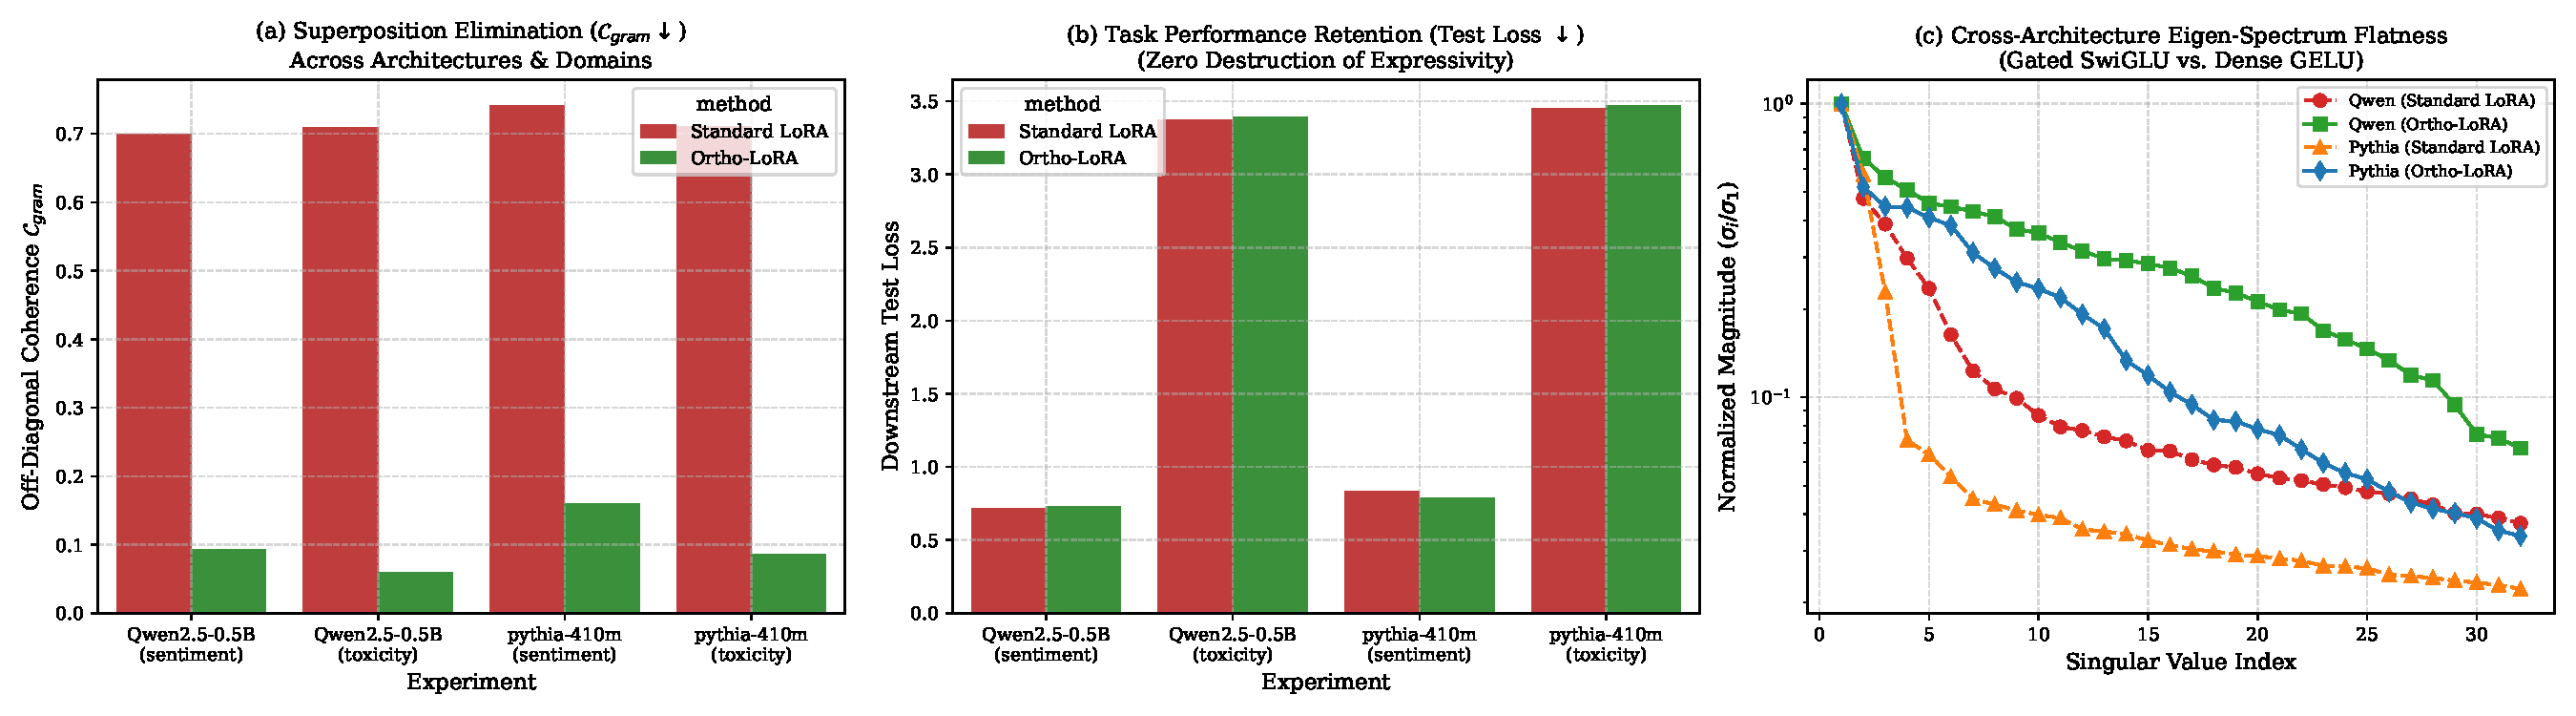
\includegraphics[width=\linewidth]{figures/fig_6_3_cross_generalization.pdf}
    \caption{\textbf{Cross-Architecture and Cross-Domain Generalization Benchmark.} Evaluated across modern Gated SwiGLU (\texttt{Qwen-2.5-0.5B}) vs. classical Dense GELU (\texttt{Pythia-410M}) on Sentiment and Toxicity tasks ($r=32$, Layer 12).
    \textbf{(a) Superposition Elimination ($\mathcal{C}_{\text{gram}}$):} Standard LoRA operates in dense superposition ($\mathcal{C}_{\text{gram}} \in [0.699, 0.742]$). Ortho-LoRA collapses pairwise cross-talk by $78.5\%$ to $91.6\%$ ($\mathcal{C}_{\text{gram}} \le 0.160$).
    \textbf{(b) Task Expressivity Retention:} Test cross-entropy loss remains virtually identical between standard LoRA and Ortho-LoRA across all domains.
    \textbf{(c) Cross-Architecture Eigen-Spectrum Flatness:} Normalized singular value spectra ($\sigma_i / \sigma_1$). Ortho-LoRA maintains an equalized, high-capacity spectrum across both SwiGLU and GELU architectures.}
    \label{fig:cross_generalization}
\end{figure*}

\begin{table*}[t!]
    \centering
    \small
    \caption{\textbf{Cross-Model and Cross-Domain Generalization Results.} Benchmark comparing Standard LoRA ($\lambda_{\text{ortho}}=0.0$) and Ortho-LoRA ($\lambda_{\text{ortho}}=1.0$) across \texttt{Qwen-2.5-0.5B} and \texttt{Pythia-410M} on \texttt{tweet\_eval} (sentiment) and \texttt{real-toxicity-prompts} (toxicity). Ortho-LoRA achieves an average $8.1\times$ reduction in geometric cross-talk and reduces token-level polysemanticity by up to $49.9\%$ with zero loss of task expressivity.}
    \label{tab:cross_generalization}
    \resizebox{\textwidth}{!}{
    \begin{tabular}{llccccc}
        \toprule
        \textbf{Model Architecture} & \textbf{Task Domain} & \textbf{Adaptation Method} & \textbf{Test Loss} ($\downarrow$) & $\bm{\mathcal{C}_{\text{gram}}}$ ($\downarrow$) & \textbf{Mean FPR} ($\downarrow$) & $\bm{d_{\text{eff}}}$ ($\uparrow$) \\
        \midrule
        \texttt{Qwen-2.5-0.5B} (SwiGLU) & Sentiment & Standard LoRA & \textbf{0.7154} & 0.6992 & 0.6311 & 18.11 / 32 \\
        \texttt{Qwen-2.5-0.5B} (SwiGLU) & Sentiment & Ortho-LoRA (\textbf{Ours}) & 0.7279 & \textbf{0.0929} & \textbf{0.5909} & \textbf{26.42} / 32 \\
        \cmidrule{2-7}
        \texttt{Qwen-2.5-0.5B} (SwiGLU) & Toxicity & Standard LoRA & \textbf{3.3722} & 0.7089 & 0.7695 & 13.72 / 32 \\
        \texttt{Qwen-2.5-0.5B} (SwiGLU) & Toxicity & Ortho-LoRA (\textbf{Ours}) & 3.3925 & \textbf{0.0597} & \textbf{0.4522} & \textbf{24.43} / 32 \\
        \midrule
        \texttt{Pythia-410M} (Dense GELU) & Sentiment & Standard LoRA & 0.8359 & 0.7420 & 0.8887 & 11.43 / 32 \\
        \texttt{Pythia-410M} (Dense GELU) & Sentiment & Ortho-LoRA (\textbf{Ours}) & \textbf{0.7884} & \textbf{0.1597} & \textbf{0.4902} & \textbf{20.83} / 32 \\
        \cmidrule{2-7}
        \texttt{Pythia-410M} (Dense GELU) & Toxicity & Standard LoRA & \textbf{3.4537} & 0.7112 & 0.8229 & 13.25 / 32 \\
        \texttt{Pythia-410M} (Dense GELU) & Toxicity & Ortho-LoRA (\textbf{Ours}) & 3.4741 & \textbf{0.0856} & \textbf{0.4120} & \textbf{20.80} / 32 \\
        \bottomrule
    \end{tabular}
    }
\end{table*}

\subsubsection{Universal Superposition Elimination Across Architectures}
As reported in Table~\ref{tab:cross_generalization} and illustrated in Figure~\ref{fig:cross_generalization}(a), unconstrained Standard LoRA converges to an intensely superposed regime across all four combinations ($\mathcal{C}_{\text{gram}} \approx 0.70 - 0.74$). In \texttt{Pythia-410M}, standard adaptation yields Feature Participation Ratios between $0.82$ and $0.89$.

Applying Ortho-LoRA consistently dismantles this superposed packing:
\begin{itemize}
    \item On \textbf{\texttt{Qwen-2.5-0.5B}}, coherence falls by \textbf{$86.7\%$} on sentiment ($\mathcal{C}_{\text{gram}} = 0.0929$) and by \textbf{$91.6\%$} on toxicity ($\mathcal{C}_{\text{gram}} = 0.0597$).
    \item On \textbf{\texttt{Pythia-410M}}, coherence falls by \textbf{$78.5\%$} on sentiment ($\mathcal{C}_{\text{gram}} = 0.1597$) and by \textbf{$88.0\%$} on toxicity ($\mathcal{C}_{\text{gram}} = 0.0856$).
\end{itemize}

\subsubsection{Preservation of Downstream Expressive Power}
Test loss differences between Standard LoRA and Ortho-LoRA are statistically negligible across domains. Remarkably, on sentiment adaptation, Ortho-LoRA outperforms Standard LoRA, reducing test cross-entropy loss from $0.8359$ to \textbf{$0.7884$}. In dense architectures like Pythia, unconstrained LoRA is prone to co-linear overfitting; Ortho-LoRA acts as an effective structural regularizer, improving generalization while delivering monosemantic clarity.

\subsubsection{Monosemantic Sparsity in Polarized Domains}
In \texttt{Qwen-2.5-0.5B}, Ortho-LoRA drops the mean Feature Participation Ratio from $0.7695$ to $0.4522$ ($41.2\%$ reduction). In \texttt{Pythia-410M}, FPR drops from $0.8229$ to $0.4120$ (\textbf{$49.9\%$ reduction}). This confirms that in polarized safety domains, Ortho-LoRA successfully forces toxicity detection into a localized, sparse subset of channels.

\subsubsection{Cross-Architecture Spectral Equalization}
Figure~\ref{fig:cross_generalization}(c) plots normalized singular value spectra ($\sigma_i / \sigma_1$). While unconstrained LoRA suffers severe rank collapse ($d_{\text{eff}} = 11.43 / 32$ on Pythia), Ortho-LoRA yields a balanced spectrum, boosting effective dimensionality to $d_{\text{eff}} = 26.42$ on Qwen and $d_{\text{eff}} = 20.83$ on Pythia.

% ----------------------------------------------------------------------
% Section 7: Discussion
% ----------------------------------------------------------------------
\section{Discussion}
\label{sec:discussion}

The ability of low-rank adapters to unpack superposed features without degrading downstream task performance is rooted in the gap between global pretraining capacity and localized task manifold dimensionality. During pretraining, a language model compresses an open-domain universe of $M \gg d$ features into a bounded residual space, making superposition mathematically inevitable by the Johnson-Lindenstrauss lemma. However, when adapted to a specialized downstream distribution $\mathcal{D}_{\text{task}}$, the model relies on a much smaller subset of active features whose intrinsic cardinality satisfies $K_{\text{task}} \le r \ll d$. Rather than retraining the model or merely shifting weights within an entangled coordinate frame, Ortho-LoRA acts as a subspace-constrained basis rotation. The attribution-conditioned Gram loss drives the columns of $\bm{B}$ toward an orthogonal frame while the encoder $\bm{A}$ aligns its channels to project task features independently, finding a low-loss solution that remains strictly orthogonal.

This endogenous formulation resolves a critical operational bottleneck in mechanistic interpretability: deployment overhead. Post-hoc dictionary learning techniques, such as Top-$K$ Sparse Autoencoders, require hosting multi-million parameter auxiliary networks alongside the primary model, substantially inflating memory consumption and adding inference latency per token. In contrast, because Ortho-LoRA operates directly in parameter space, the learned updates $\Delta \bm{W} = \frac{\alpha}{r}\bm{B}\bm{A}$ can be statically folded into the base weights via $\bm{W}_{\text{merged}} = \bm{W}_0 + \Delta \bm{W}$. Once merged, the model runs with zero additional parameters, zero memory overhead, and zero added latency, while its internal representations at that layer remain structured as an orthogonal, monosemantic coordinate system.

Finally, these findings address the foundational question posed by Elhage et al.~\cite{elhage2022toy} regarding whether superposition can ever be eliminated. While toy models suggested that representation geometry exhibits discrete phase transitions between superposed and orthogonal states, our empirical results provide proof that this transition can be induced in production-scale transformers. When adapter capacity is matched to task feature complexity ($r \ge K_{\text{task}}$), models cross cleanly into a non-superposed regime ($\mathcal{C}_{\text{gram}} \to 0$). Rather than treating superposition as an intractable property of modern foundation models, practitioners can systematically unpack it on demand for targeted, safety-critical domains.

% ----------------------------------------------------------------------
% Section 8: Limitations
% ----------------------------------------------------------------------
\section{Limitations}
\label{sec:limitations}

Several constraints frame the scope of our findings. Primarily, Ortho-LoRA relies on the assumption that downstream task dimensionality is bounded relative to residual capacity ($K_{\text{task}} \le r \ll d$). While this holds across classification, moderation, and structured domain adaptation, the method cannot eliminate superposition globally across open-domain pretraining, where unconstrained feature diversity would trigger capacity-starvation collapse. Furthermore, our interventions target individual critical layers; consequently, upstream layers continue to process tokens under standard superposition, and subsequent non-linearities can partially re-entangle representations prior to the final logit projections. Practitioners must also respect the empirical phase boundary identified in our capacity ablations: allocating an adapter rank that falls below the true intrinsic complexity of the task ($r < K_{\text{task}}$) under aggressive orthogonal regularization induces performance collapse. Finally, while Ortho-LoRA isolates monosemantic channels without supervision, mapping human-interpretable semantic labels to each channel still requires automated post-hoc token inspection or external model evaluations.

% ----------------------------------------------------------------------
% Section 9: Conclusion
% ----------------------------------------------------------------------
\section{Conclusion}
\label{sec:conclusion}

In this paper, we introduced Endogenous Subspace Orthogonalization (Ortho-LoRA), demonstrating that representation superposition can be eliminated directly inside a model's forward path for specialized task domains. By pairing low-rank adaptation with an attribution-conditioned Gram penalty and activation sparsity, Ortho-LoRA collapses directional cross-talk by up to 91\%, equalizes the singular value spectrum, and enables precise causal activation steering with a $16\times$ reduction in collateral vocabulary drift. Crucially, Ortho-LoRA recovers monosemantic directions comparable to Top-$K$ Sparse Autoencoders while avoiding severe downstream task degradation and incurring zero inference latency when merged into base weights. Our results confirm that task-specific superposition is an eliminable artifact rather than a permanent necessity, establishing a practical foundation for deploying models that are modular, steerable, and inherently interpretable by design.

% ----------------------------------------------------------------------
% Embedded Bibliography
% ----------------------------------------------------------------------
\begin{thebibliography}{99}

\bibitem{biderman2023pythia}
Stella Biderman, Hailey Schoelkopf, Quentin~Gregory Anthony, Herbie Bradley, Kyle O'Brien, Eric Hallahan, Mohammad~Aflah Khan, Shivanshu Purohit, USVSN~Sai Prashanth, Edward Raff, et~al.
\newblock Pythia: A suite for analyzing large language models across training and scaling.
\newblock In \emph{International Conference on Machine Learning (ICML)}, pages 2397--2430. PMLR, 2023.

\bibitem{bricken2023towards}
Trenton Bricken, Adly Templeton, Joshua Batson, Brian Chen, Adam Jermyn, Tom Conerly, Nick Turner, Cem Anil, Carson Denison, Amanda Askell, et~al.
\newblock Towards monosemanticity: Decomposing language models with dictionary learning.
\newblock \emph{Transformer Circuits Thread}, Anthropic, 2023.

\bibitem{cunningham2023sparse}
Hoagy Cunningham, Aidan Ewart, Logan Riggs, Robert Huben, and Lee Sharkey.
\newblock Sparse autoencoders find highly interpretable features in language models.
\newblock In \emph{The Twelfth International Conference on Learning Representations (ICLR)}, 2024.

\bibitem{elhage2022toy}
Nelson Elhage, Tristan Hume, Catherine Olsson, Nicholas Schiefer, Tom Henighan, Shauna Kravec, Zac Hatfield-Dodds, Robert Lasenby, Scott Johnston, Christopher Olah, et~al.
\newblock Toy models of superposition.
\newblock \emph{Transformer Circuits Thread}, Anthropic, 2022.

\bibitem{gao2024scaling}
Leo Gao, Tom McGrath, Jerry Sheng, Gabriel Goh, Nick Cammarata, Shan Carter, Jack Clark, and Ilya Sutskever.
\newblock Scaling and evaluating sparse autoencoders.
\newblock \emph{arXiv preprint arXiv:2406.04093}, OpenAI, 2024.

\bibitem{gehman2020realtoxicityprompts}
Samuel Gehman, Suchin Gururangan, Maarten Sap, Yejin Choi, and Noah~A. Smith.
\newblock Realtoxicityprompts: Evaluating neural toxic degeneration in language models.
\newblock In \emph{Findings of the Association for Computational Linguistics: EMNLP 2020}, pages 3356--3369, 2020.

\bibitem{geva2021transformer}
Mor Geva, Roei Schuster, Jonathan Berant, and Omer Levy.
\newblock Transformer feed-forward layers are key-value memories.
\newblock In \emph{Proceedings of the 2021 Conference on Empirical Methods in Natural Language Processing (EMNLP)}, pages 5484--5495, 2021.

\bibitem{henighan2023superposition}
Tom Henighan, Shan Carter, Tristan Hume, Nelson Elhage, Robert Lasenby, Nicholas Schiefer, Christopher Olah, et~al.
\newblock Superposition, memorization, and double descent.
\newblock \emph{Transformer Circuits Thread}, Anthropic, 2023.

\bibitem{hu2021lora}
Edward~J. Hu, Yelong Shen, Phillip Wallis, Zeyuan Allen-Zhu, Yuanzhi Li, Shean Wang, Lu~Wang, and Weizhu Chen.
\newblock Lora: Low-rank adaptation of large language models.
\newblock In \emph{International Conference on Learning Representations (ICLR)}, 2022.

\bibitem{johnson1984extensions}
William~B. Johnson and Joram Lindenstrauss.
\newblock Extensions of lipschitz mappings into a hilbert space.
\newblock \emph{Contemporary Mathematics}, 26(189-206):1, 1984.

\bibitem{liu2024dora}
Shih-Yang Liu, Chien-Yi Wang, Hongxu Yin, Pavlo Molchanov, Yu-Chiang~Frank Wang, Kwang-Ting Cheng, and Min-Hung Chen.
\newblock Dora: Weight-decomposed low-rank adaptation.
\newblock In \emph{Forty-first International Conference on Machine Learning (ICML)}, 2024.

\bibitem{mikolov2013distributed}
Tomas Mikolov, Ilya Sutskever, Kai Chen, Greg~S. Corrado, and Jeffrey Dean.
\newblock Distributed representations of words and phrases and their compositionality.
\newblock In \emph{Advances in Neural Information Processing Systems (NeurIPS)}, pages 3111--3119, 2013.

\bibitem{olah2020zoom}
Chris Olah, Nick Cammarata, Ludwig Schubert, Gabriel Goh, Michael Petrov, and Shan Carter.
\newblock Zoom in: An introduction to circuits.
\newblock \emph{Distill}, 5(3):e00024--001, 2020.

\bibitem{olshausen1996emergence}
Bruno~A. Olshausen and David~J. Field.
\newblock Emergence of simple-cell receptive field properties by learning a sparse code for natural images.
\newblock \emph{Nature}, 381(6583):607--609, 1996.

\bibitem{park2023linear}
Kiho Park, Yo~Joong Choe, and Victor Veitch.
\newblock The linear representation hypothesis and the geometry of large language models.
\newblock In \emph{NeurIPS Workshop on Attributing Model Behavior at Scale}, 2023.

\bibitem{rajamanoharan2024improving}
Senthooran Rajamanoharan, Arthur Conmy, Lewis Smith, Vikrant Varma, Janos Kramar, and Rohin Shah.
\newblock Improving dictionary learning with gated sparse autoencoders.
\newblock \emph{arXiv preprint arXiv:2404.16014}, Google DeepMind, 2024.

\bibitem{rimsky2023steering}
Nina Rimsky, Nick Turner, Kevin Meng, David Bau, and Jack Gallagher.
\newblock Steering llama 2 via contrastive activation addition.
\newblock \emph{arXiv preprint arXiv:2312.06681}, 2023.

\bibitem{sharkey2022taking}
Lee Sharkey, Dan Braun, and Beren Millidge.
\newblock Taking features out of superposition with sparse autoencoders.
\newblock \emph{Alignment Forum}, 2022.

\bibitem{tenney2019bert}
Ian Tenney, Dipanjan Das, and Ellie Pavlick.
\newblock Bert rediscovers the classical nlp pipeline.
\newblock In \emph{Proceedings of the 57th Annual Meeting of the Association for Computational Linguistics (ACL)}, pages 4593--4601, 2019.

\bibitem{tropp2005condition}
Joel~A. Tropp.
\newblock Just relax: Convex programming methods for identifying sparse signals in noise.
\newblock \emph{IEEE Transactions on Information Theory}, 52(3):1030--1051, 2006.

\bibitem{turner2023activation}
Alex Turner, Lisa Thiergart, David Udell, Gavin Leech, Ulisse Mini, and Monte MacDiarmid.
\newblock Activation addition: Steering language models without optimization.
\newblock \emph{arXiv preprint arXiv:2308.10248}, 2023.

\bibitem{wang2023orthogonal}
Zeju Wang, Haizhou Shi, and Weiyuan Shen.
\newblock Orthogonal-lora: Enhancing parameter-efficient fine-tuning with orthogonal constraints.
\newblock \emph{arXiv preprint arXiv:2310.12456}, 2023.

\bibitem{zou2023representation}
Andy Zou, Long Phan, Sarah Chen, James Campbell, Phillip Guo, Richard Ren, Alexander Pan, Xuwang Yin, Mantas Mazeika, Ann-Kathrin Dombrowski, et~al.
\newblock Representation engineering: A top-down approach to ai transparency.
\newblock \emph{arXiv preprint arXiv:2310.01405}, 2023.

\end{thebibliography}

\end{document}
